\chapter{Results and Discussion}
\label{sec:results}
This chapter will present the results of denoising the different datasets, and discuss the quality of the results. For the three different datasets introduced in \cref{sec:method:datasets}, different parts of the denoising will be analysed. 

For the borosilicate glass spheres dataset, the focus has been on how much noise can be removed, what effect changing the loss function has on the denoising, and what effect the pre-processing steps have on the denoising. 

The soda lime glass spheres dataset denoising has focused on comparing TomoGAN denoising to \gls{piccs} reconstruction denoising, and how well the denoising captures 3D information. 

Finally, the Pierre shale dataset has been used to explore the possibilities of using TomoGAN to denoise when a corresponding high-quality dataset is unavailable. 

\section{Borosilicate Glass Spheres}
In this section, denoising of the borosilicate glass spheres dataset (see \cref{sec:method:datasets:tomo00058}) from TomoBank has been explored. On this dataset, the effect of the depth parameter of TomoGAN has not been explored (see \cref{sec:method:tomogan}), instead focus has been on how much noise can be removed, and the effects of pre-processing and changing the loss function for training.

\subsection{Denoising with Different Amounts of Noise}
To explore the efficiency of the denoising method, the borosilicate glass spheres dataset was reconstructed with four different levels of projection undersampling. By using subsampling factors of $8$, $16$, $32$, and $48$ (see \cref{tab:projectionsubsampling}), four datasets with different levels of artifacting were simulated. They are given alongside the \gls{hq} reconstruction in \cref{fig:tomo00058missingwedgecomparison}. 

The TomoGAN network was trained with a loss function containing \gls{mse}, log-cosh, VGG, and adversarial components, a depth of 1 was used, and the network was trained for 100000 iterations with a mini batch size of 16. The resulting denoised images are given in \cref{fig:tomo00058missingwedgecomparisondenoised}

\begin{figure}
  \begin{subfigure}[t]{\textwidth}
    \centering
    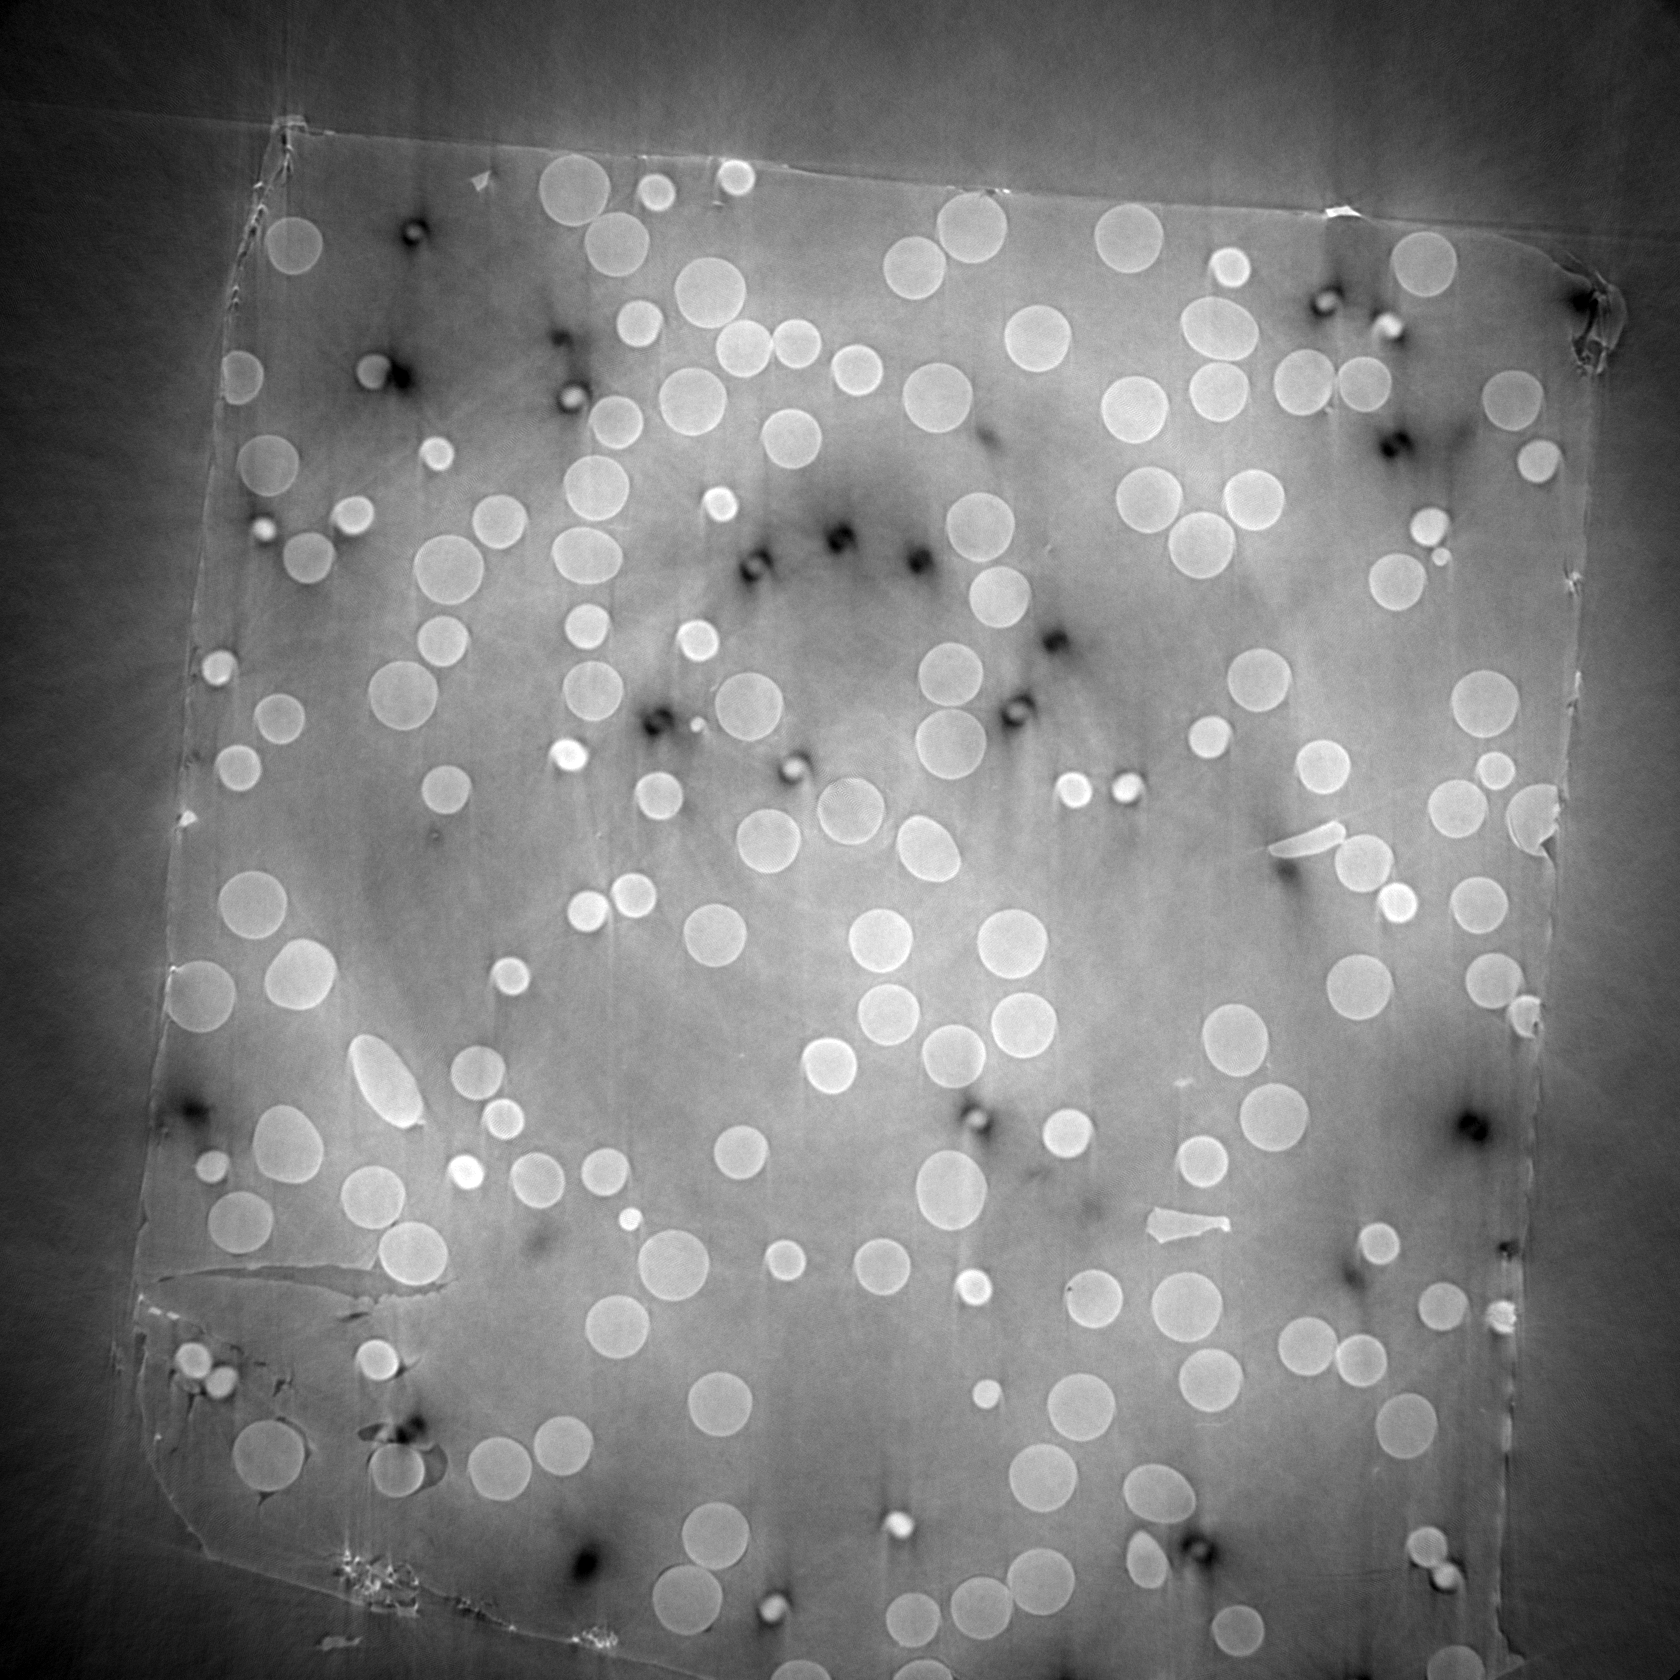
\includegraphics[width=.45\textwidth]{figures/gt32.png}
    \caption{\Gls{hq} (1500 projections). }
  \end{subfigure}

  \medskip

  \begin{subfigure}[t]{.45\textwidth}
    \centering
    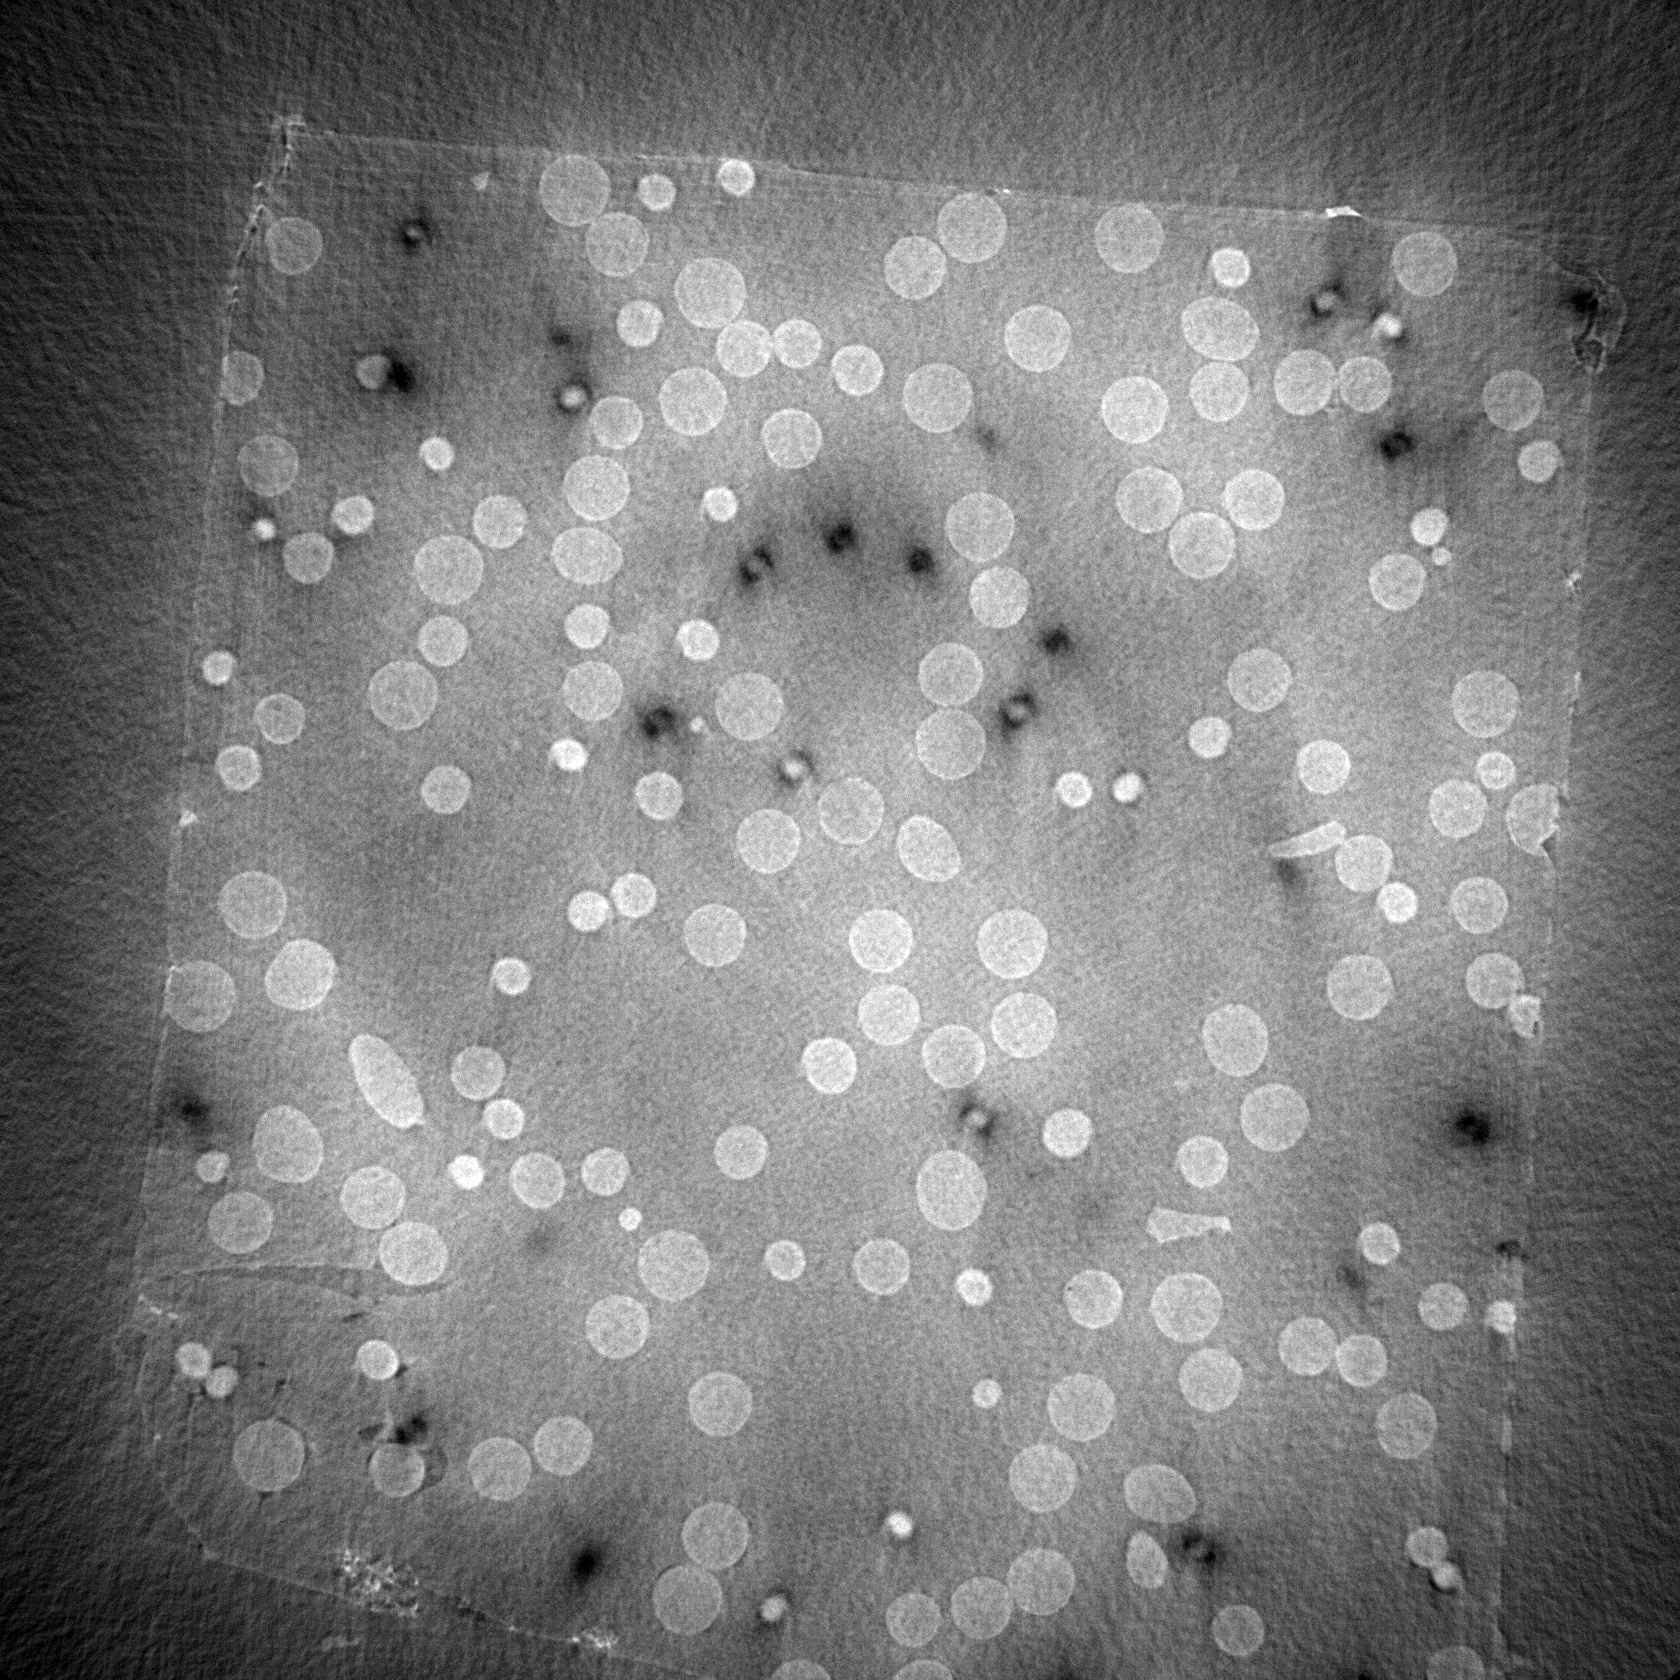
\includegraphics[width=\linewidth]{figures/ns8.png}
    \caption{Subsampling factor 8 (187 projections). }
  \end{subfigure}
  \hfill
  \begin{subfigure}[t]{.45\textwidth}
    \centering
    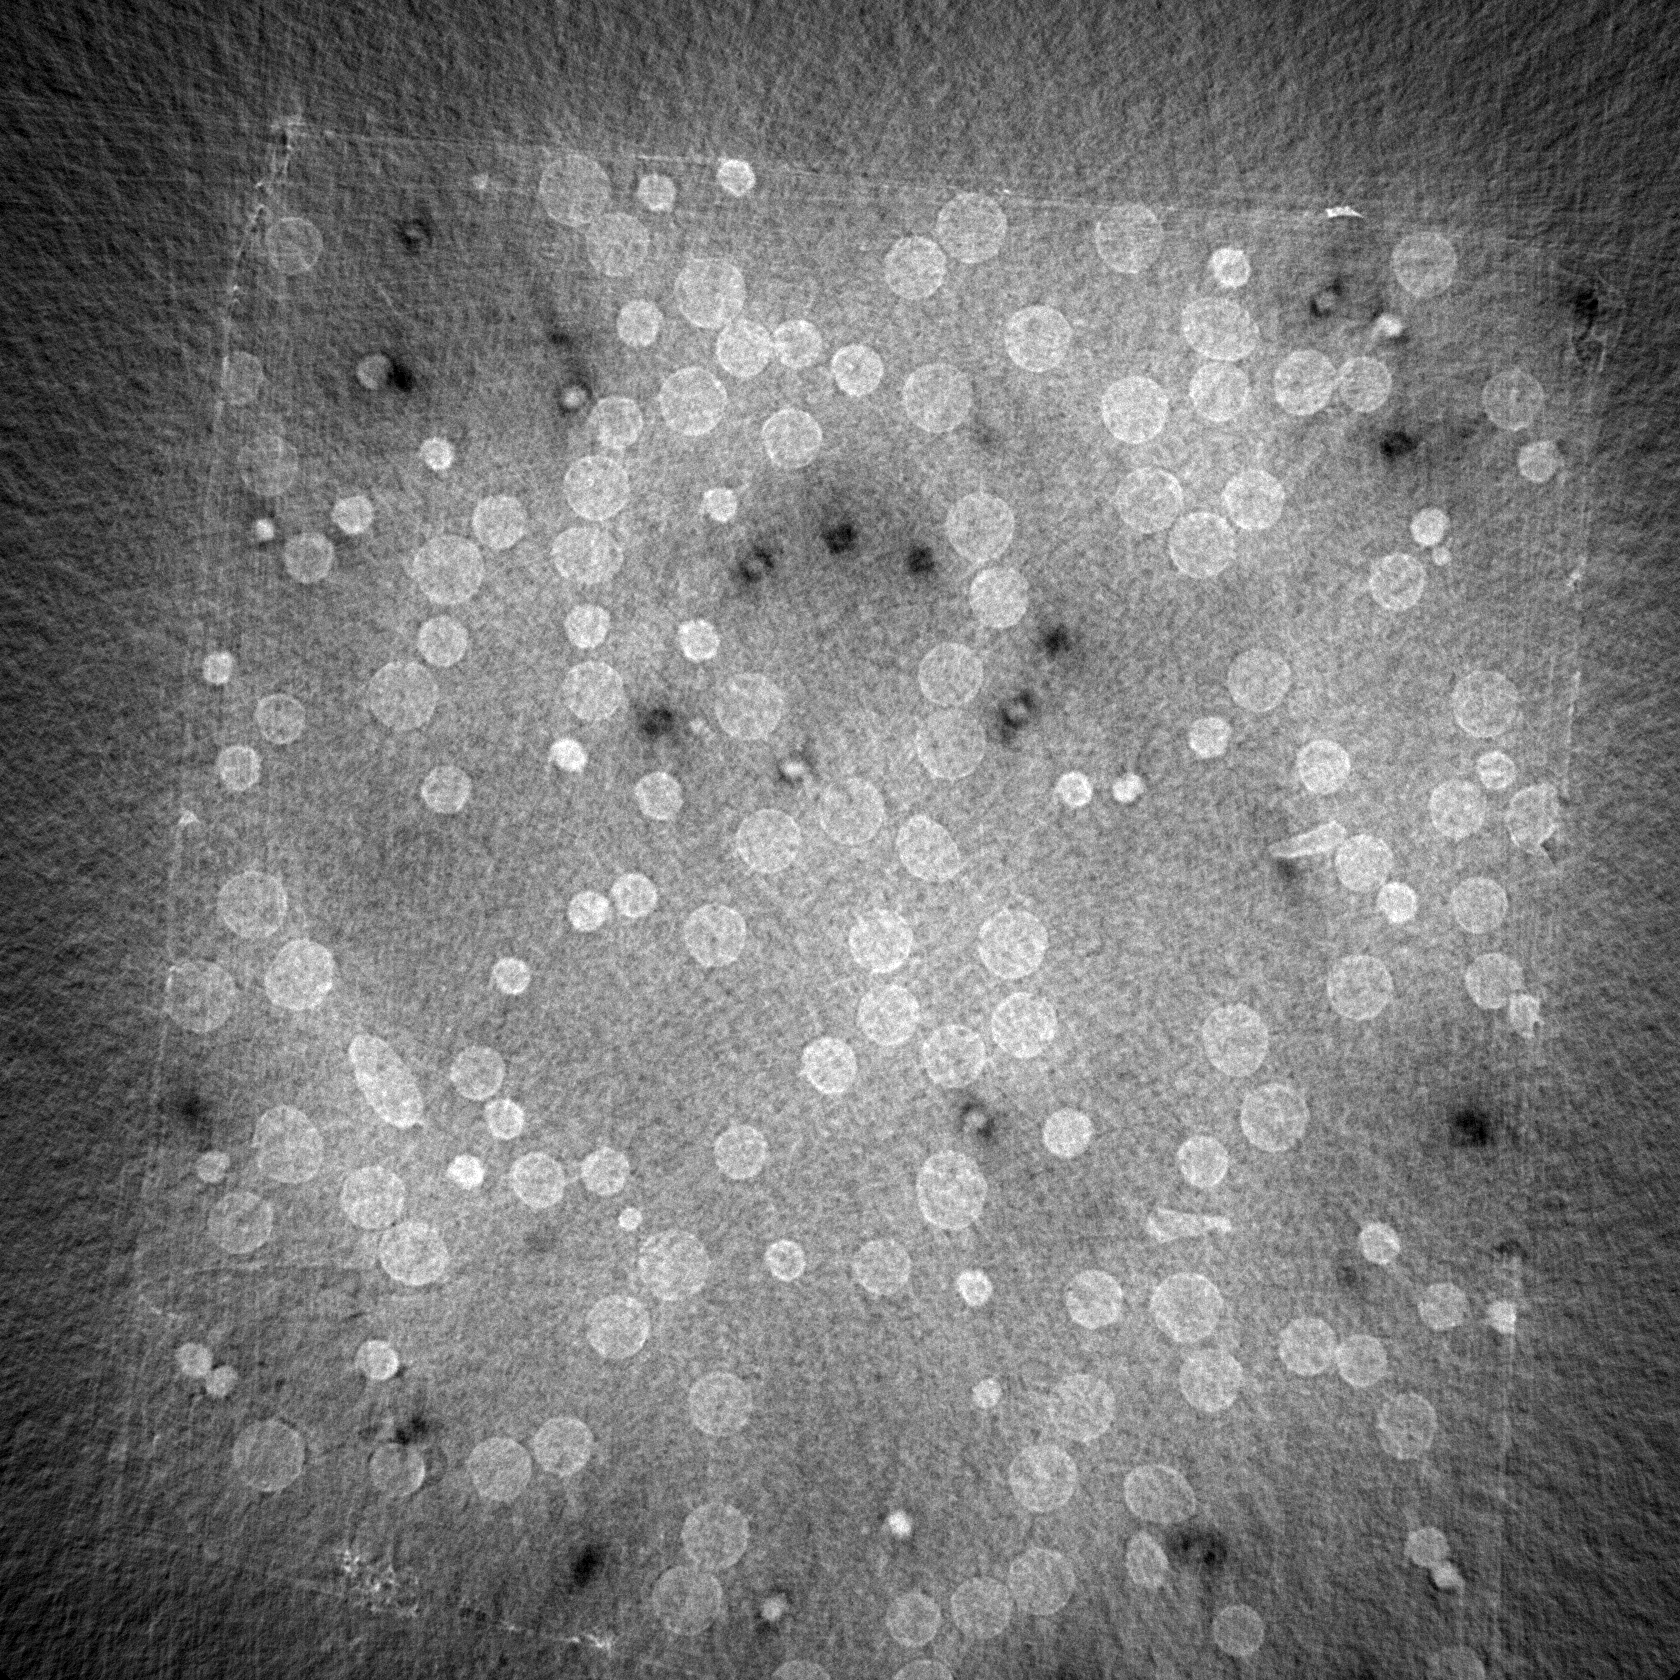
\includegraphics[width=\linewidth]{figures/ns16.png}
    \caption{Subsampling factor 16 (93 projections). }
  \end{subfigure}

  \medskip

  \begin{subfigure}[t]{.45\textwidth}
    \centering
    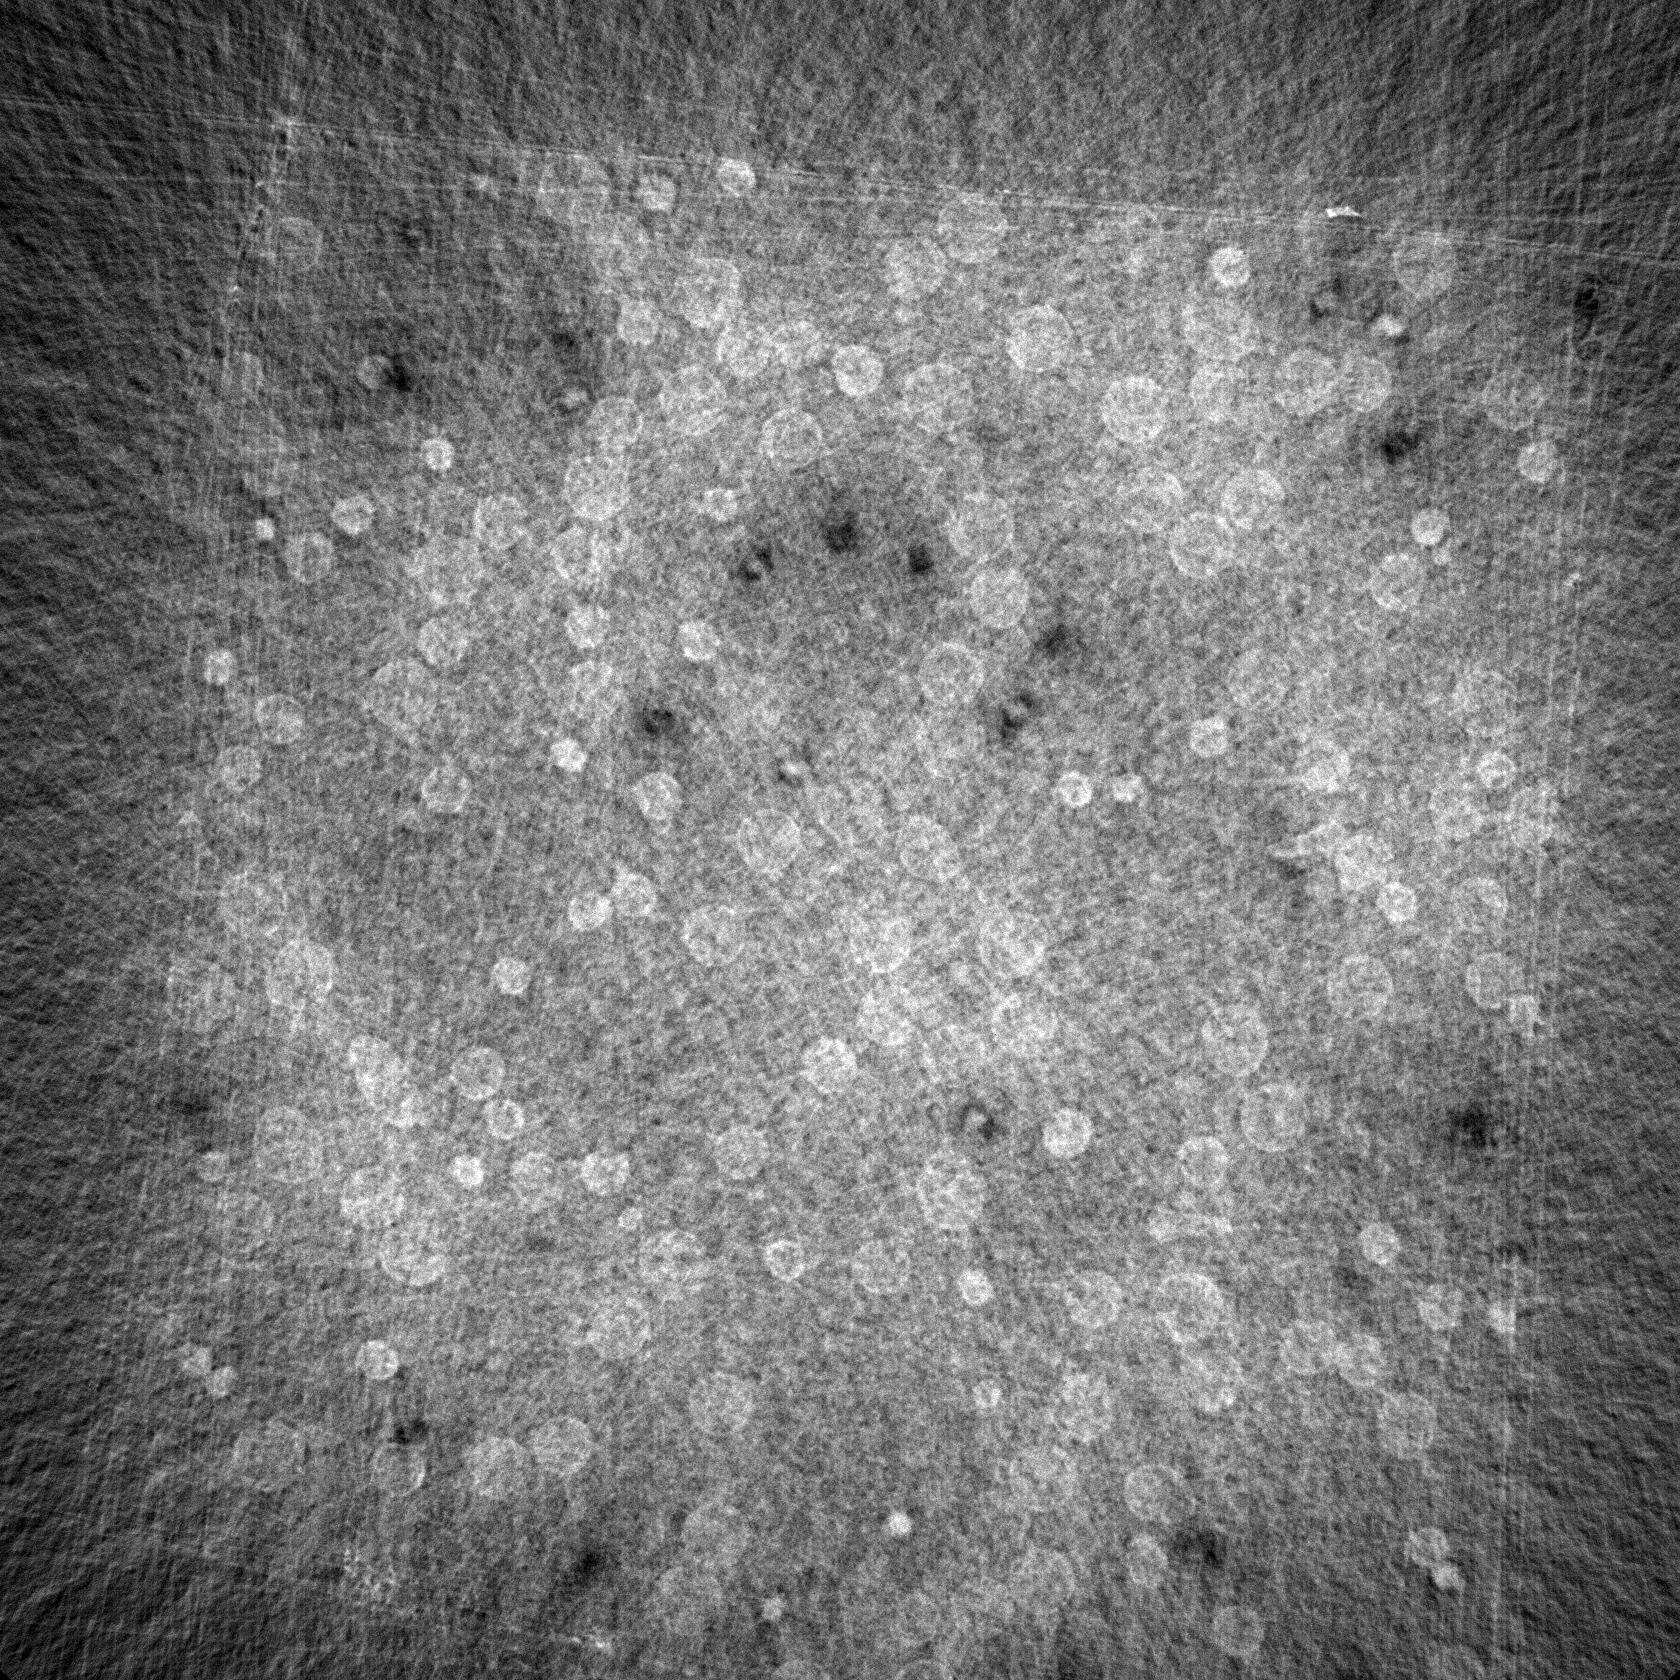
\includegraphics[width=\linewidth]{figures/ns32.png}
    \caption{Subsampling factor 32 (46 projections). }
  \end{subfigure}
  \hfill
  \begin{subfigure}[t]{.45\textwidth}
    \centering
    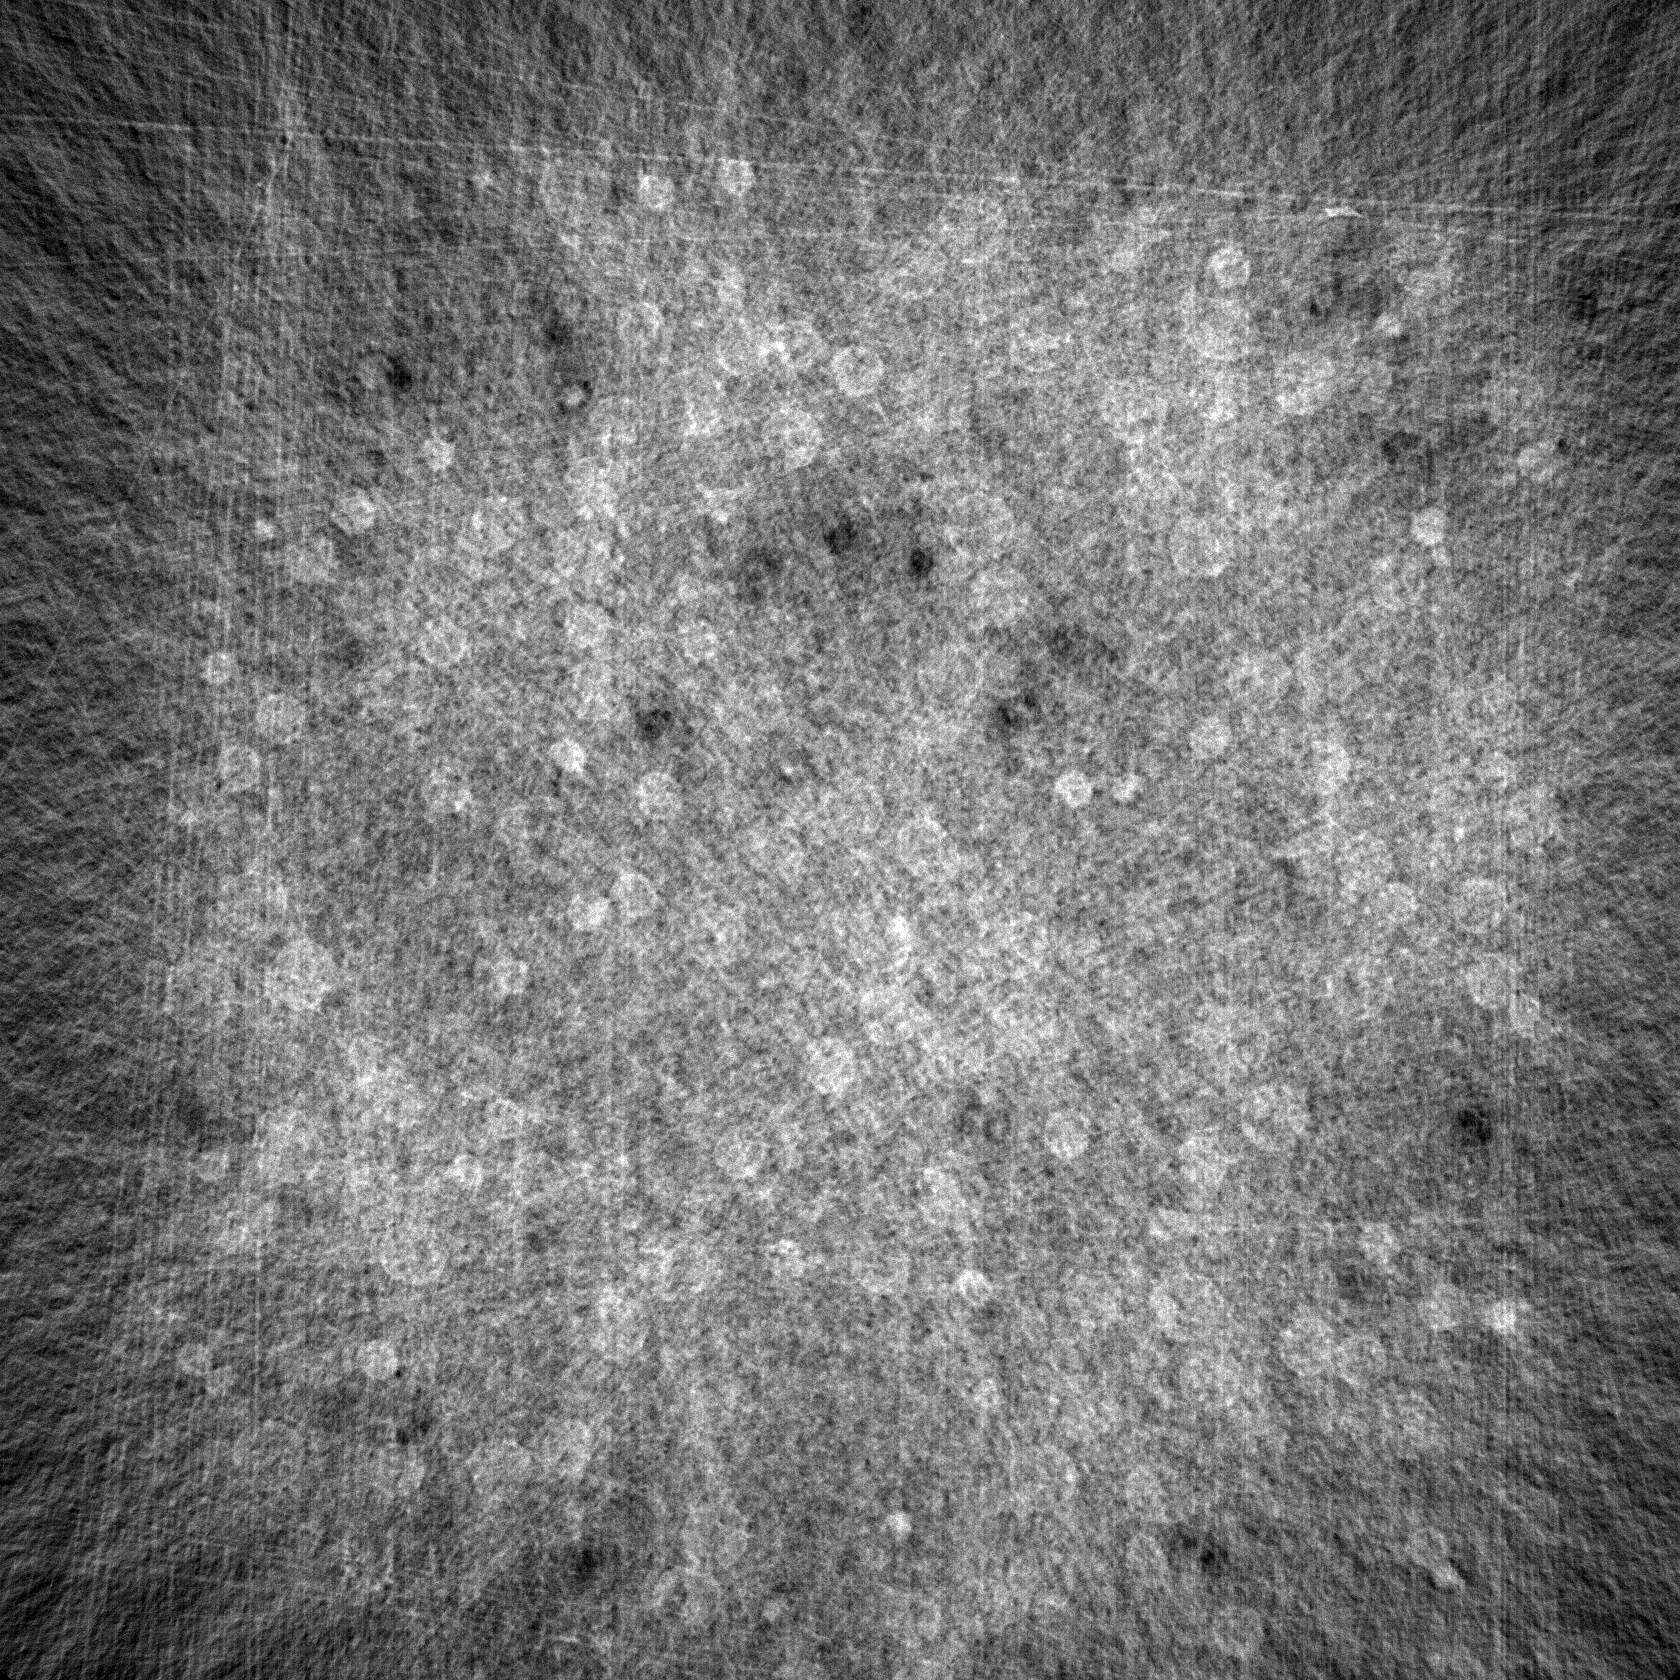
\includegraphics[width=\linewidth]{figures/ns48.png}
    \caption{Subsampling factor 48 (31 projections). }
  \end{subfigure}
  \caption[Four different levels of projection undersampling]{Comparison of different levels of projection undersampling on the borosilicate glass spheres dataset by reconstructing the images with the \gls{fbp} algorithm. The same cross-section is displayed for different reconstructions made by varying the number of projections used.  }
  \label{fig:tomo00058missingwedgecomparison}
\end{figure}

\begin{figure}
  \begin{subfigure}[t]{.45\textwidth}
    \centering
    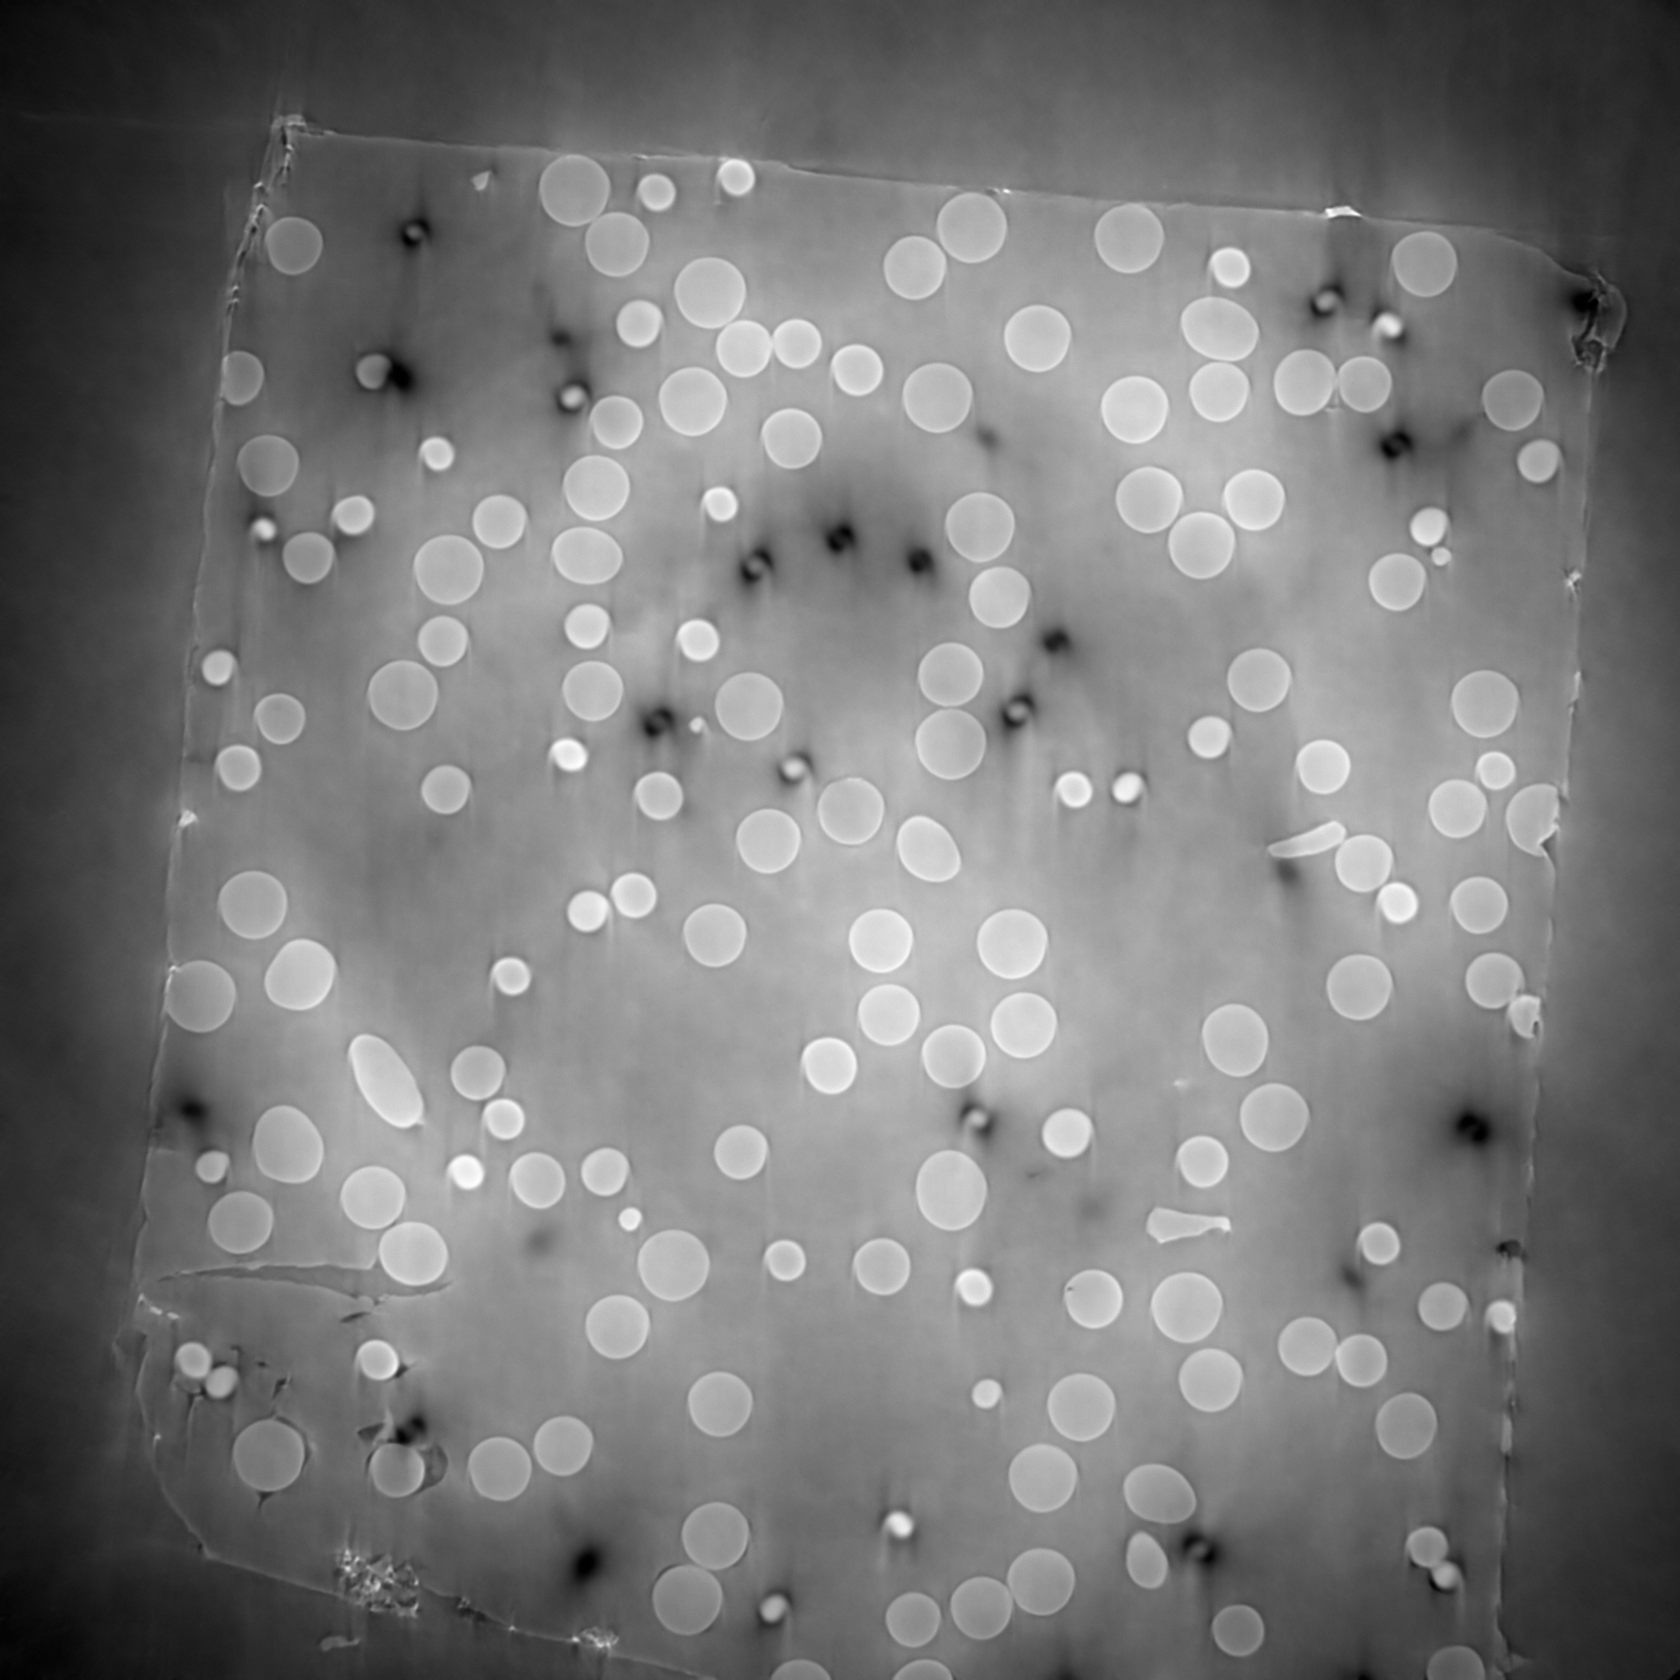
\includegraphics[width=\linewidth]{figures/ns8it100000itd4mse035logcosh3.png}
    \caption{Subsampling factor 8 (187 projections). }
  \end{subfigure}
  \hfill
  \begin{subfigure}[t]{.45\textwidth}
    \centering
    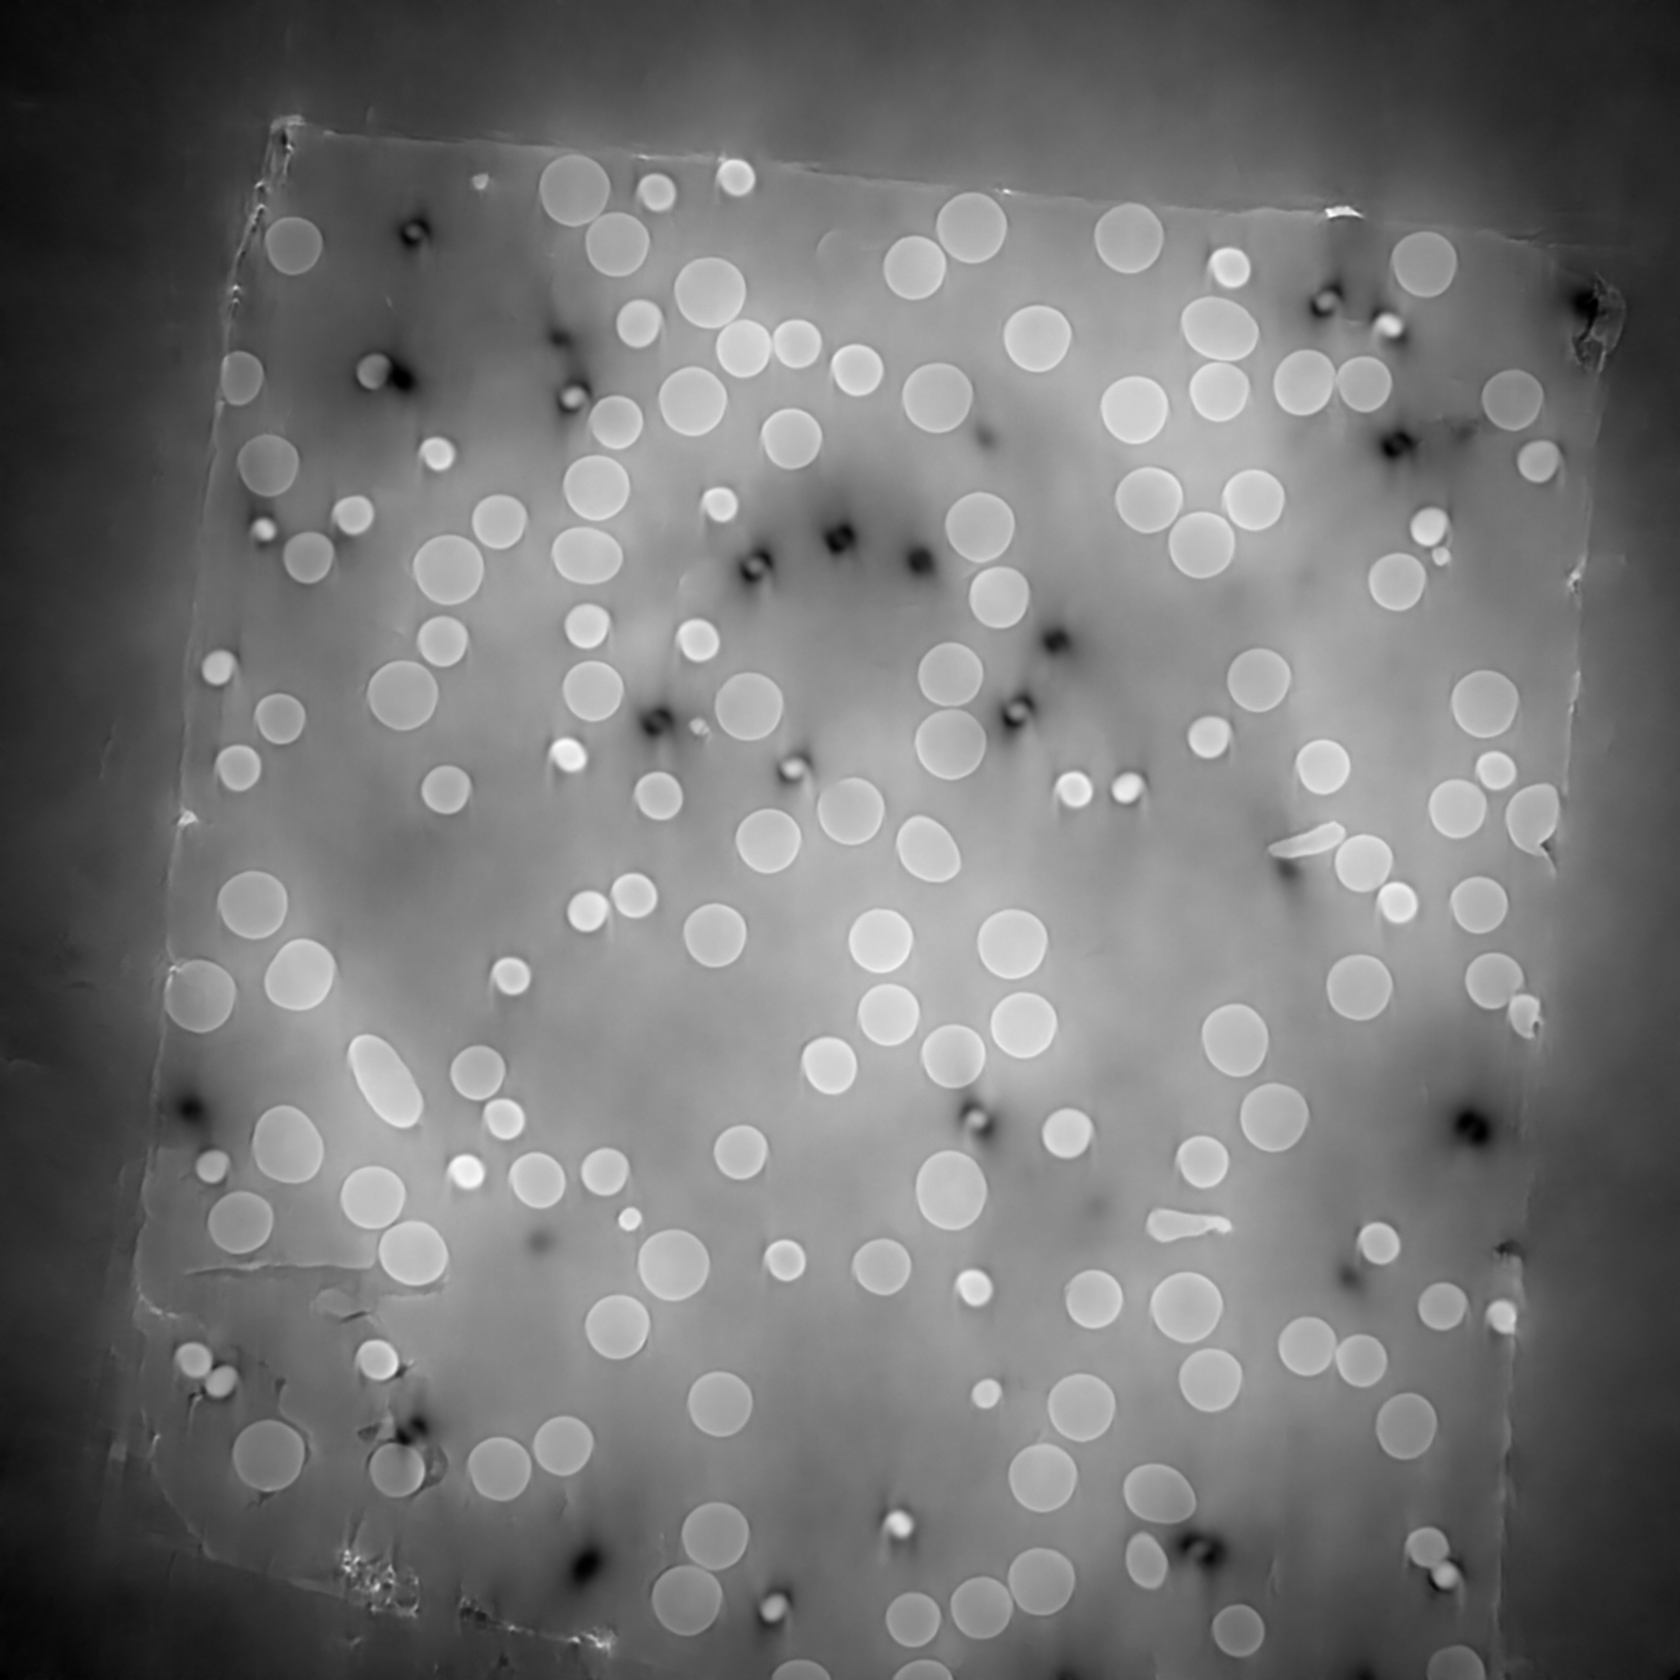
\includegraphics[width=\linewidth]{figures/ns16it100000itd4mse035logcosh3.png}
    \caption{Subsampling factor 16 (93 projections). }
  \end{subfigure}

  \medskip

  \begin{subfigure}[t]{.45\textwidth}
    \centering
    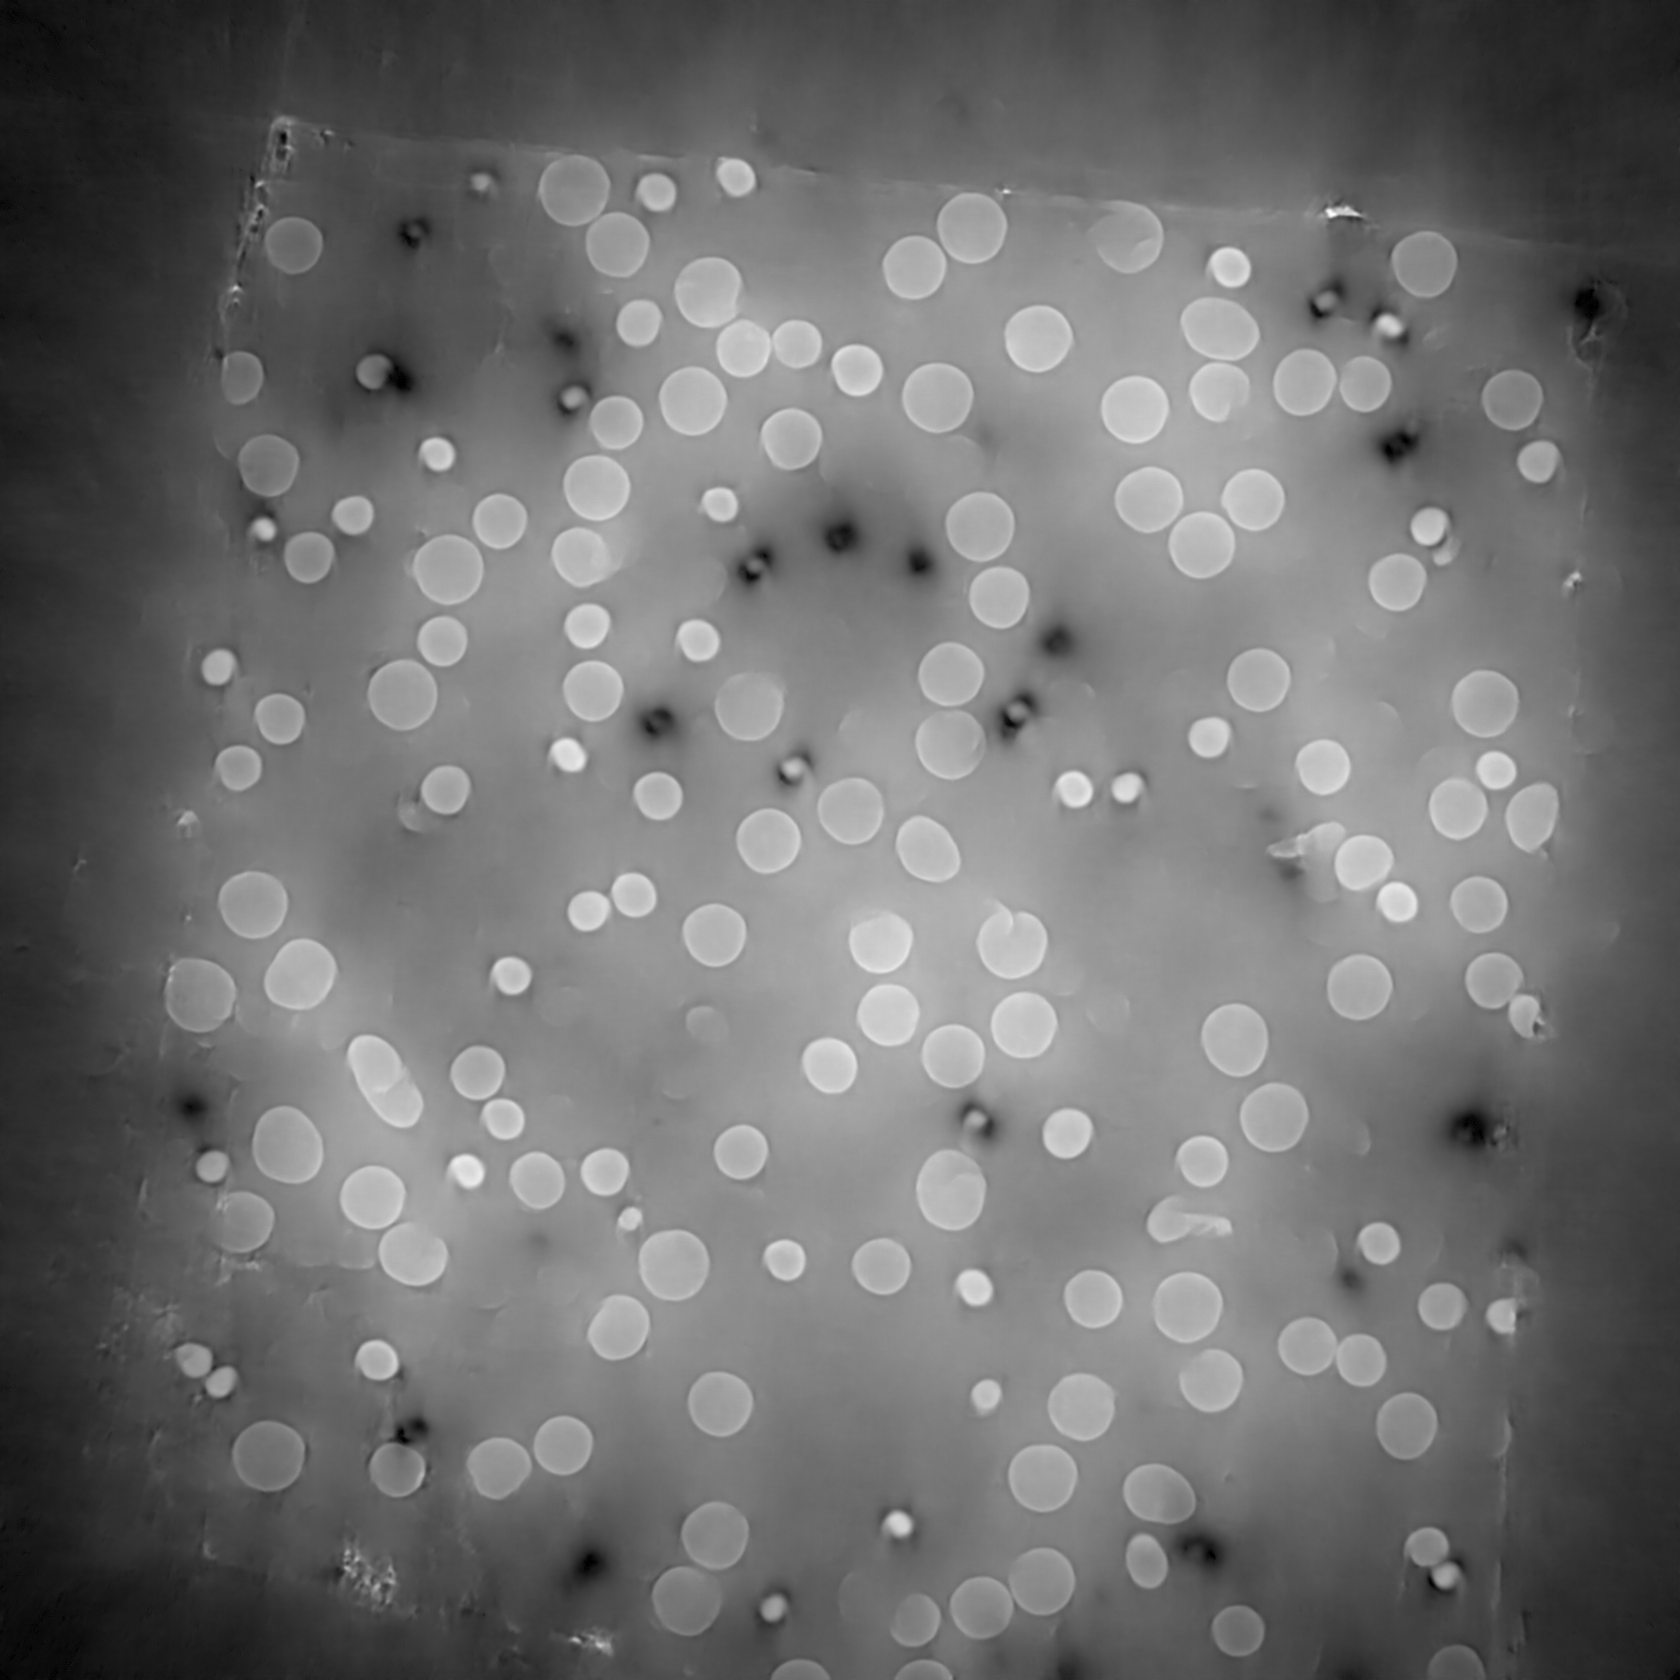
\includegraphics[width=\linewidth]{figures/ns32it100000itd4mse035logcosh3.png}
    \caption{Subsampling factor 32 (46 projections). }
  \end{subfigure}
  \hfill
  \begin{subfigure}[t]{.45\textwidth}
    \centering
    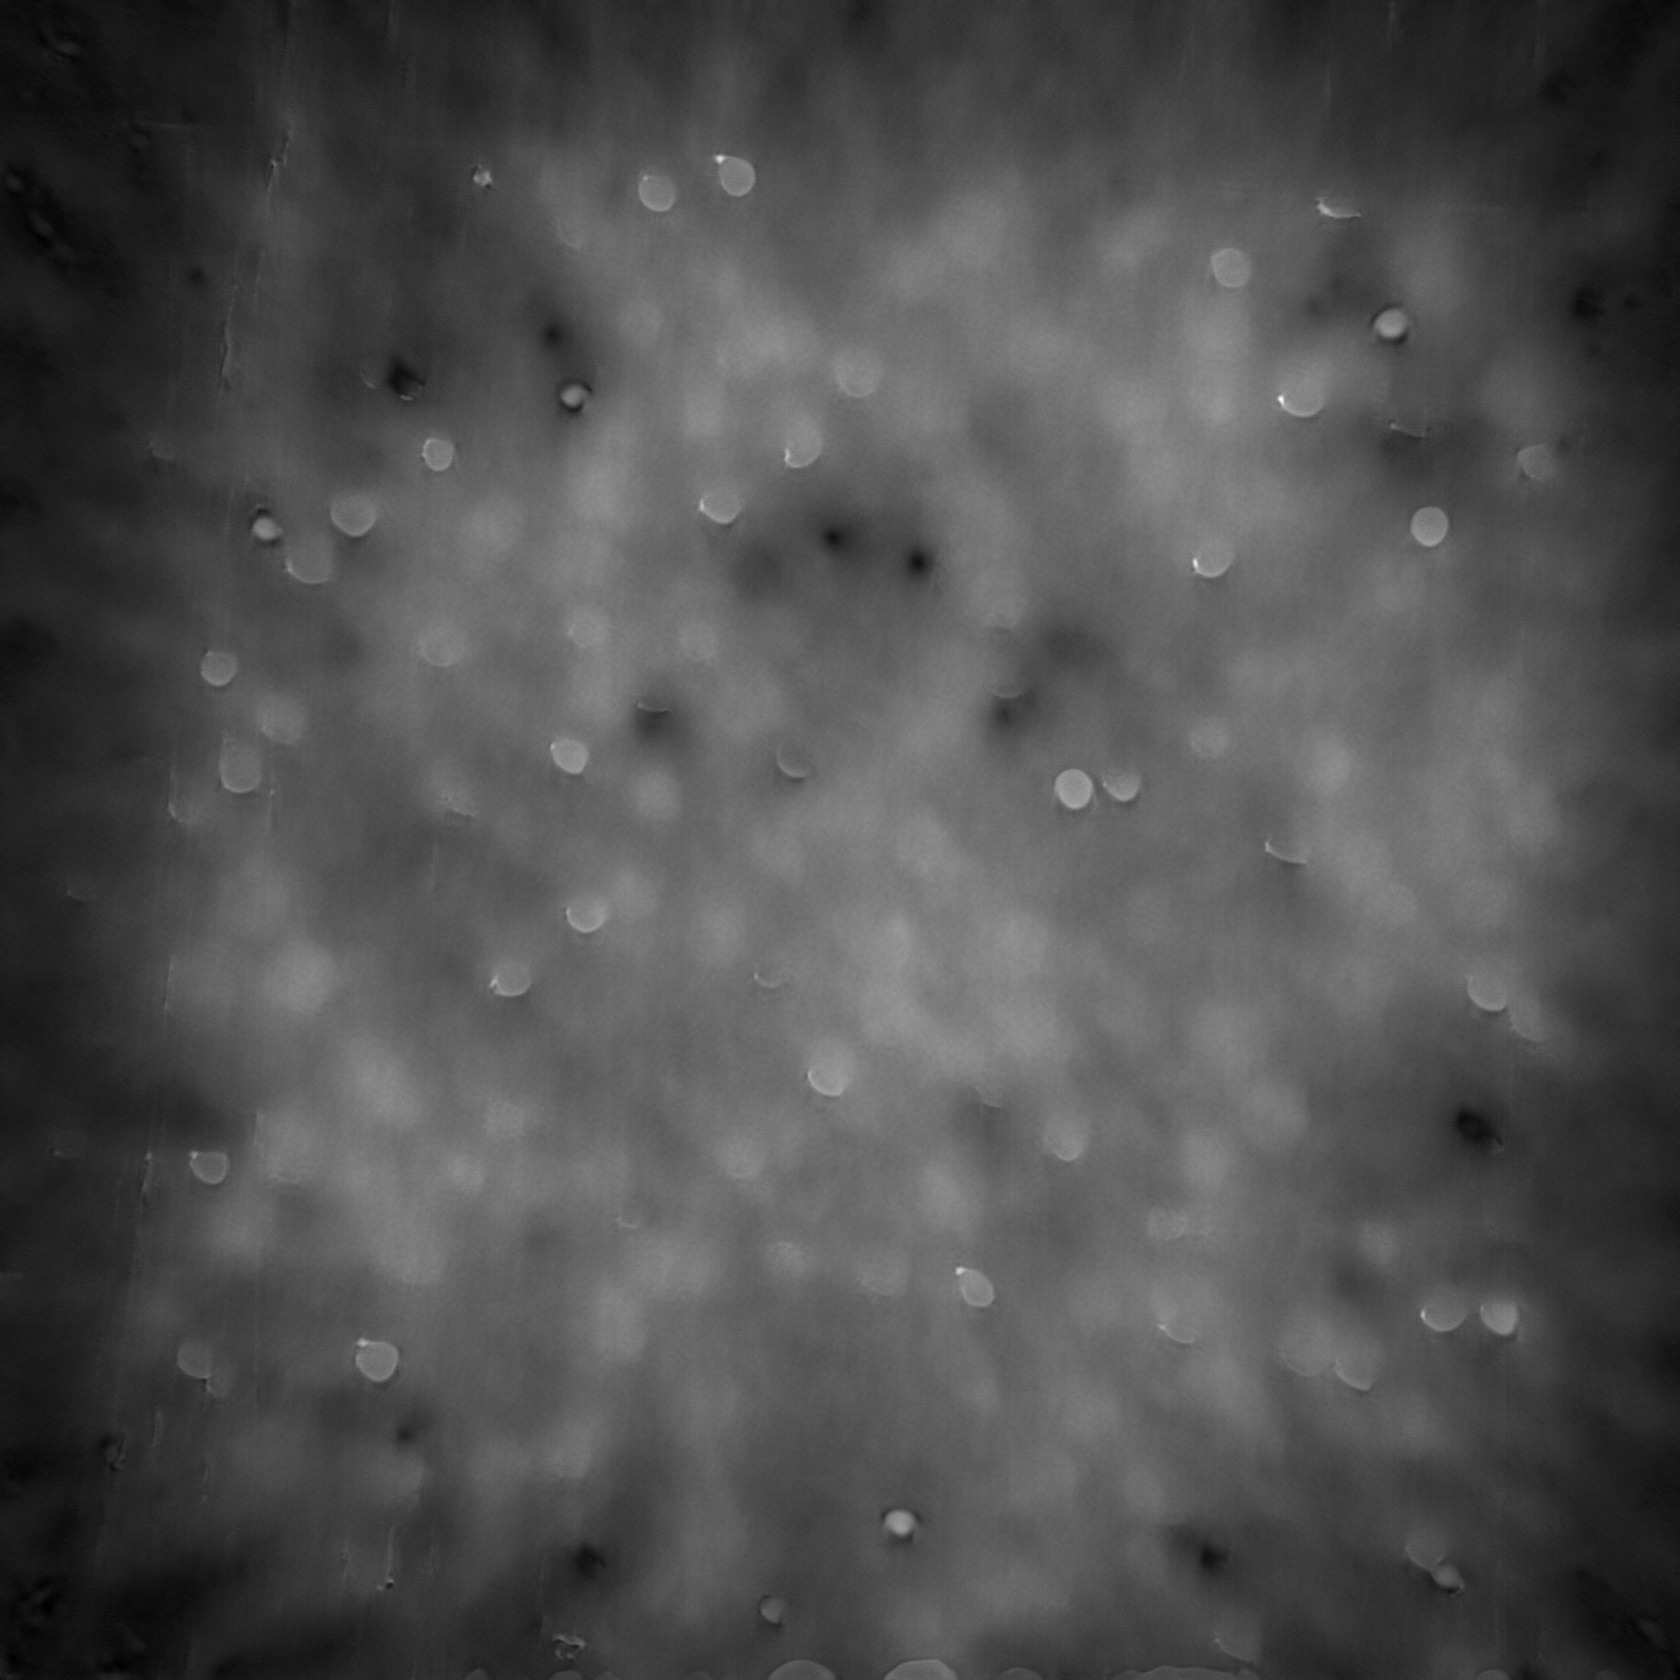
\includegraphics[width=\linewidth]{figures/ns48it100000itd4mse035logcosh3.png}
    \caption{Subsampling factor 48 (31 projections). }
  \end{subfigure}
  \caption[Denoising of four different levels of projection undersampling]{Comparison of denoising of different levels of projection undersampling on the borosilicate glass spheres dataset, where the corresponding noisy images are given in \cref{fig:tomo00058missingwedgecomparison}. The denoising was done with TomoGAN using a loss function containing \gls{mse}, log-cosh, VGG, and adversarial loss components, a depth of 1, and the network was trained for $100 000$ iterations with a mini batch size of 16. }
  \label{fig:tomo00058missingwedgecomparisondenoised}
\end{figure}

It is evident that a subsampling factor of 48, corresponding to merely 31 projections, leads to too much noise to recover any usable denoised image. This is further confirmed by looking at plots of the pixel values along two different lines on the denoised images and comparing them with the noisy and the \gls{hq} image, as is provided in \cref{fig:differentnoiselineplot1,fig:differentnoiselineplot2}. For the other three levels of undersampling the denoising seems to result in images sufficiently similar to the \gls{hq} image, especially for subsampling factors $8$ and $16$. 

\begin{figure}[htbp]
  \centering
  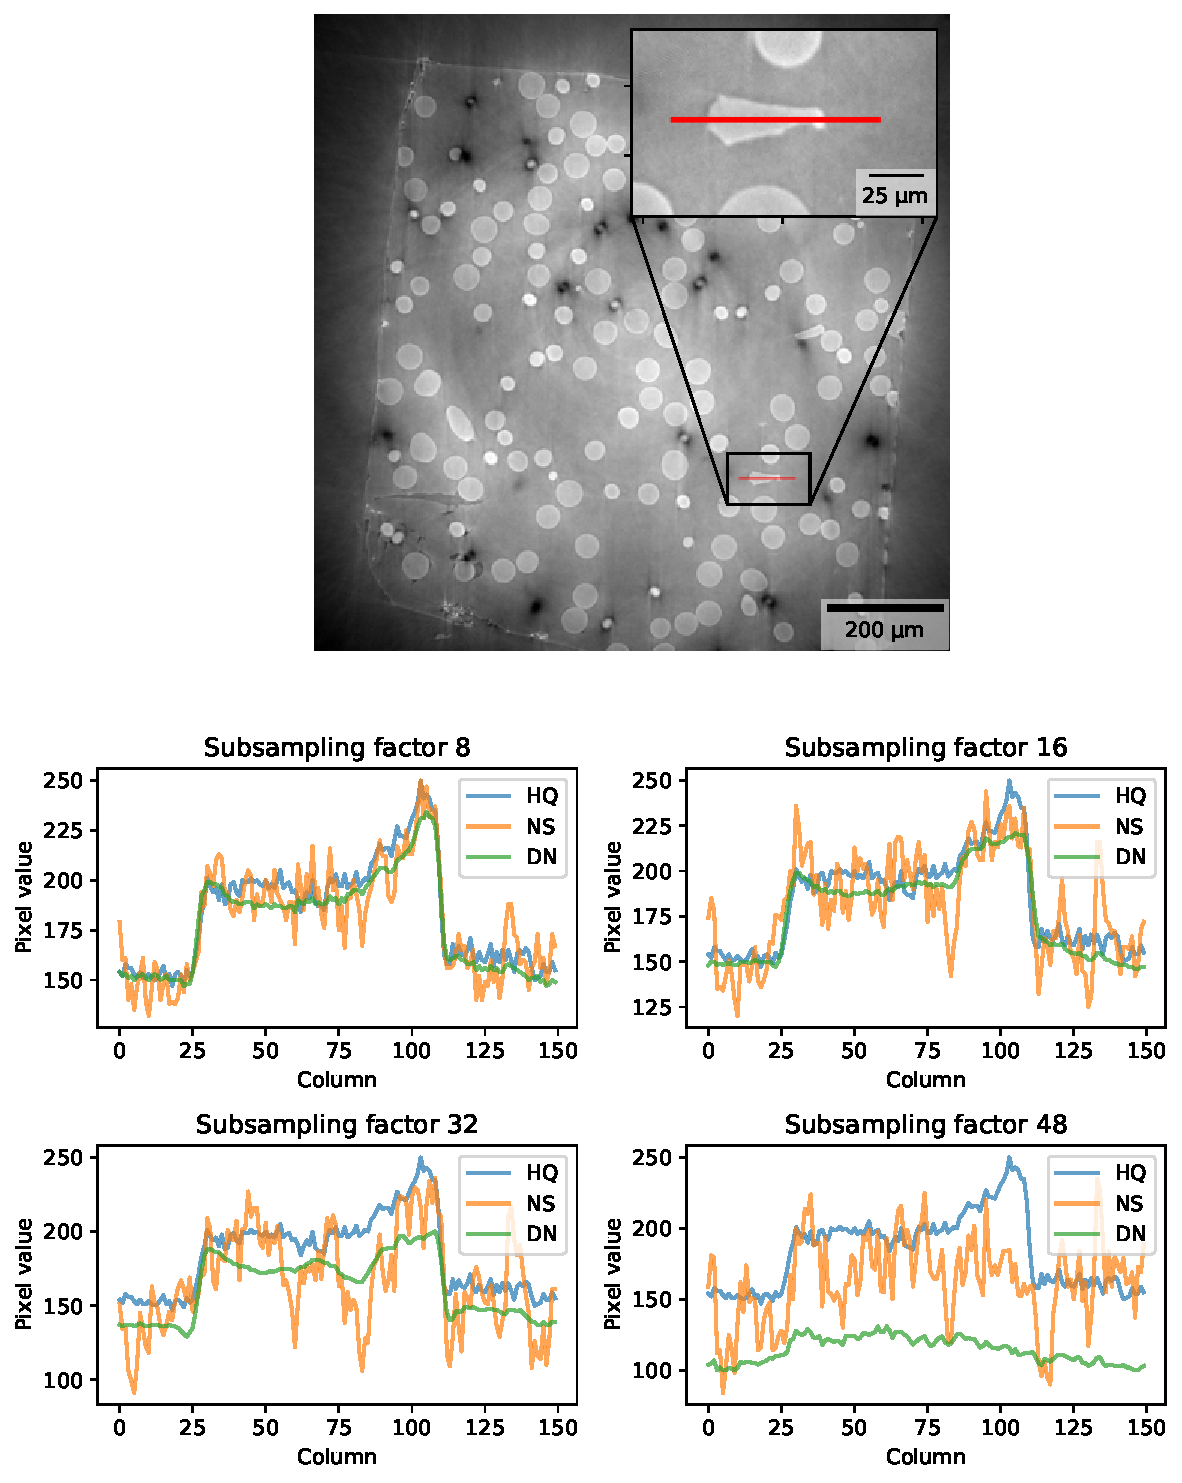
\includegraphics[width=.95\textwidth]{figures/differentnoiselineplot1.pdf}
  \caption[Pixel value plot of denoising of different levels of projection undersampling on the borosilicate glass spheres dataset]{The plots show pixel values for 150 pixels on a horizontal line on the borosilicate glass spheres dataset, as shown by the red line on the \gls{hq} image above, for denoising of four different levels of projection undersampling. \gls{hq} corresponds to the \gls{hq} image, NS to the noisy/low-quality image, and DN to the denoised image. The denoising was done with TomoGAN using a loss function containing \gls{mse}, log-cosh, VGG, and adversarial loss components, a depth of 1, and the network was trained for $100 000$ iterations with a mini batch size of 16. }
  \label{fig:differentnoiselineplot1}
\end{figure}

\begin{figure}[htbp]
  \centering
  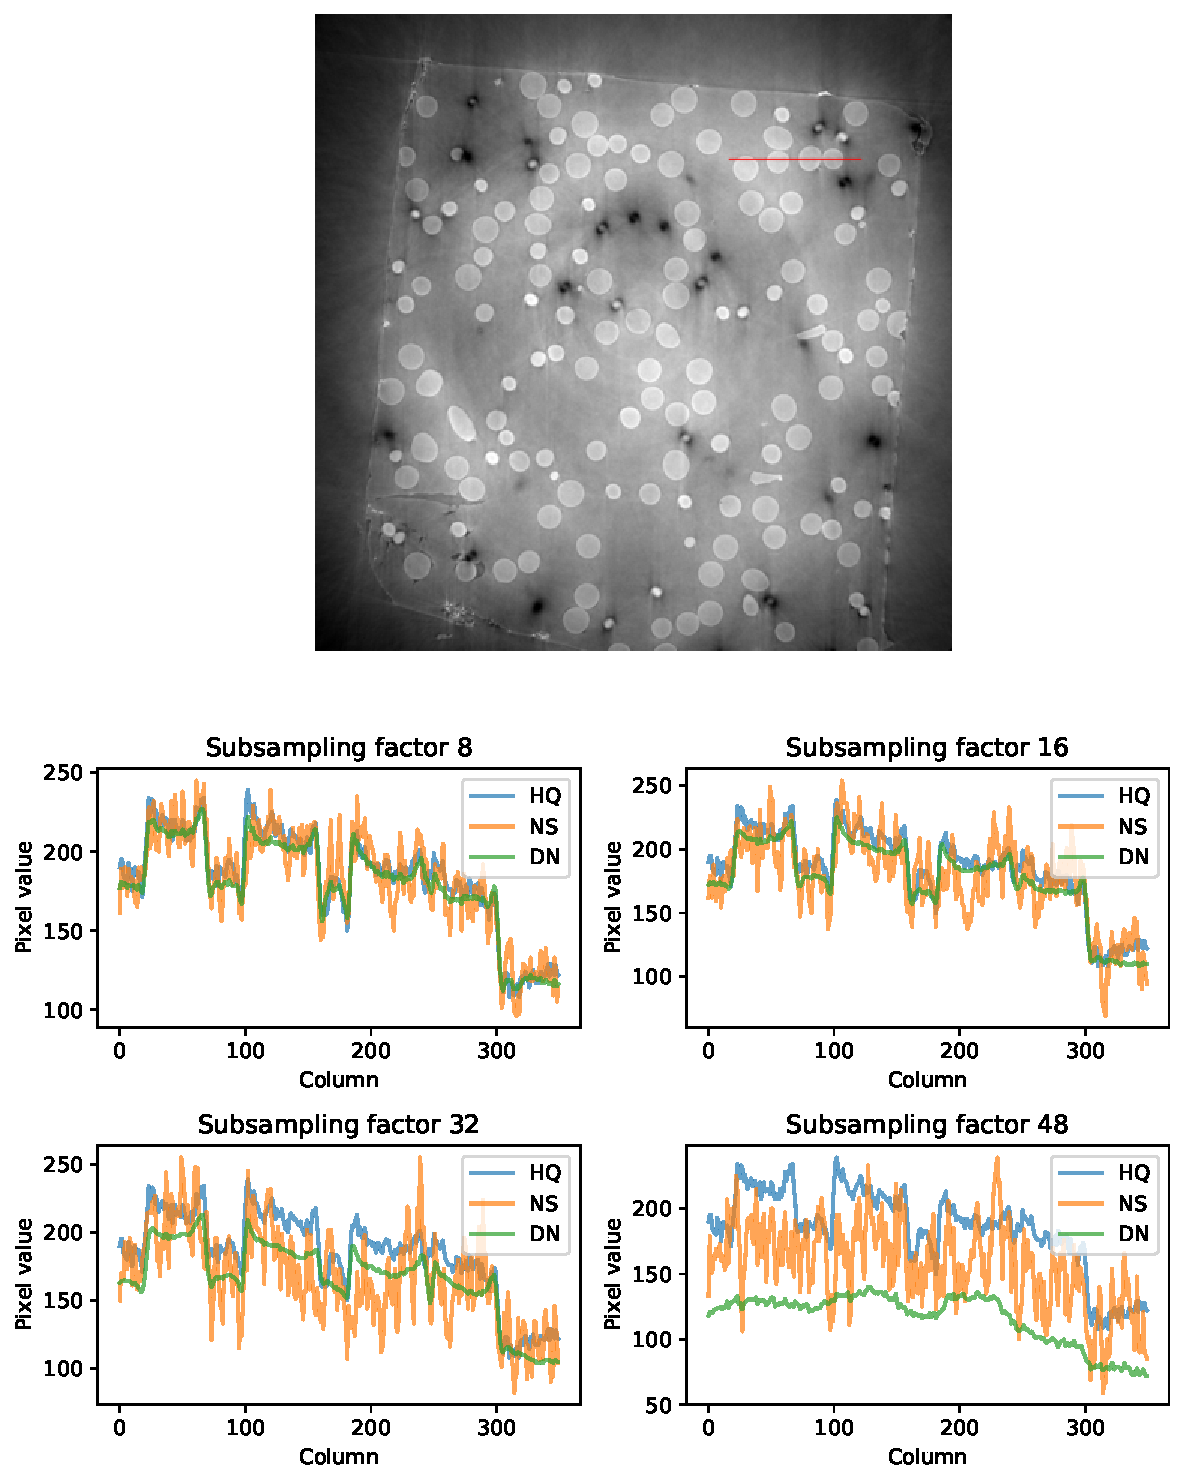
\includegraphics[width=.95\textwidth]{figures/differentnoiselineplot2.pdf}
  \caption[Pixel value plot of denoising of different levels of projection undersampling on the borosilicate glass spheres dataset]{The plots show pixel values for 400 pixels on a horizontal line on the borosilicate glass spheres dataset, as shown by the red line on the \gls{hq} image above, for denoising of four different levels of projection undersampling. Figure elements are as in \cref{fig:differentnoiselineplot1}. }
  \label{fig:differentnoiselineplot2}
\end{figure}

\cref{tab:missingwedgessim} contains \gls{ssim} and \gls{mse} values for the noisy and denoised images shown in \cref{fig:tomo00058missingwedgecomparison,fig:tomo00058missingwedgecomparisondenoised}. We see here that for subsampling factors $8$, $16$, and $32$, the \gls{mse} is improved by denoising, however for subsampling factor $48$ it is drastically worsened. All denoisings achieve, to varying degrees, \gls{ssim} improvements. The fact that the poor denoising of the subsampling factor of $48$ achieves an improvement in \gls{ssim} from $0.193$ to $0.657$ indicates that \gls{ssim} is not able to sufficiently gauge the image quality in this case. 

It is worth noting that a subsampling factor of $32$ corresponds to $46$ projections, which is similar to the $64$ projections used in the noisiest simulated dataset in the original article by Liu \textit{et al.} \cite{liu2020tomogan}. The achieved \gls{ssim} score on a real dataset of $0.789$ in this thesis is similar to their results on a simulated phantom. 

\begin{table}[htbp]
  \centering
  \caption[SSIM for different levels of simulated projection undersampling and corresponding values after denoising]{Overview of \gls{ssim} for different levels of simulated projection undersampling on the borosilicate glass spheres dataset. The projection undersampling was simulated by subsampling the number of projections by a factor as given in the subsampling factor column. All denoising was done with TomoGAN using a loss function containing \gls{mse}, log-cosh, VGG, and adversarial loss components, a depth of 1, and the network was trained for $100 000$ iterations with a mini batch size of 16. }
  \label{tab:missingwedgessim}
  \begin{tabular}{llllll}
  \hline
  \multirow{2}{*}{Subsampling factor} & \multirow{2}{*}{Projections} & \multicolumn{2}{c}{\gls{ssim}} & \multicolumn{2}{c}{\gls{mse}}  \\
  {} & {} & Noisy & Denoised & Noisy & Denoised \\
  \hhline{======}
  %\hline 
  $1$  & $1500$ & $1.0$ & $-$ & $0.0$ & $-$ \\
  $8$  & $187$ & $0.492$ & $0.842$ & $148.3$ & $33.3$ \\
  $16$ & $93$ & $0.335$ & $0.816$ & $348.5$ & $74.9$ \\
  $32$ & $46$ & $0.233$ & $0.789$ & $704.4$ & $210.8$ \\
  $48$ & $31$ & $0.193$ & $0.657$ & $976.6$ & $2362.6$ \\
  \hline
  \end{tabular}
\end{table}

\subsection{Effect of Pre-processing Images}
Attempting to denoise the borosilicate glass spheres dataset without cropping the reconstructed images yielded poor results, as can be seen in \cref{fig:uncroppeddenoising}. The network does not seem to have managed to converge properly, and the results look to simply be blurring the images. The use of an \gls{mse} based loss function may be part of the cause of the blurring, as this loss has been shown to cause blurring in image processing related tasks such as this (see \cref{sec:ml:training:lossfunctions}). 

When the images are all cropped, with no other changes being made, the network performs better. This is given in \cref{fig:croppeddenoising}. While there is artifacting from the denoising (especially when looking at shapes that differ from the common shapes in the dataset, such as non-circular shapes), when comparing the \gls{hq} and denoised images it is evident that a majority of the features have been preserved with the noise being drastically reduced. 

Comparing the non-cropped denoising with a denoising only run with a few iterations, not reaching full convergence, as seen in \cref{fig:croppednoncroppedearly}, the results are similar, indicating that the non-cropped denoising may have struggled to converge properly. 

Note that the images in \cref{fig:uncroppeddenoising,fig:croppeddenoising} have different intensity scales because of the scaling step of the preprocessing (see \cref{sec:method:compilingdataset}). 

This denoising was performed with TomoGAN using a loss function containing \gls{mse}, log-cosh, VGG, and adversarial loss components, a depth of 1, and the network was trained for 100000 iterations with a mini batch size of 16. 

\begin{figure}[htbp]
  \centering
  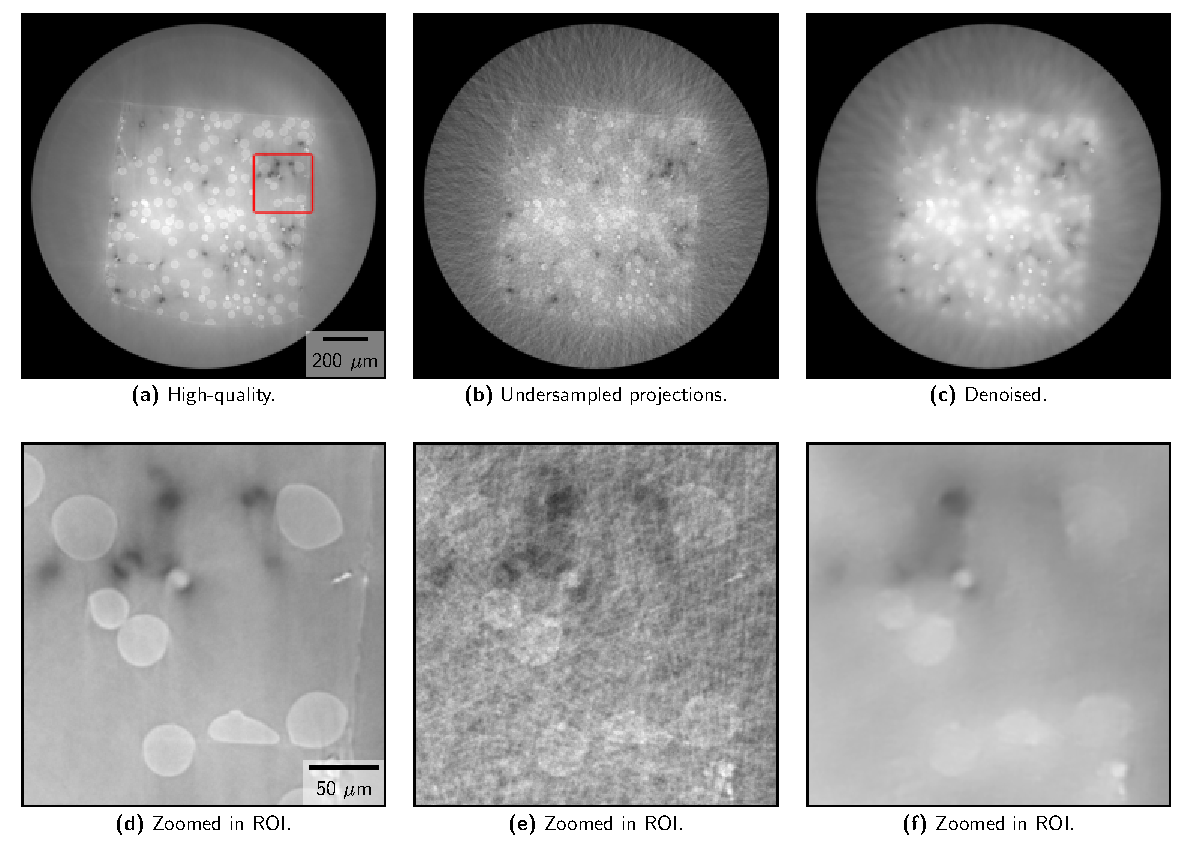
\includegraphics[width=.9\textwidth]{figures/uncroppeddenoising.pdf}
  \caption[Non-cropped image denoising]{Denoising of non-cropped borosilicate glass spheres dataset. Images d), e), and f) are zoomed in \gls{roi}s of images a), b), and c) respectively. The \gls{roi} is marked in a). }
  \label{fig:uncroppeddenoising}
\end{figure}

\begin{figure}[htbp]
  \centering
  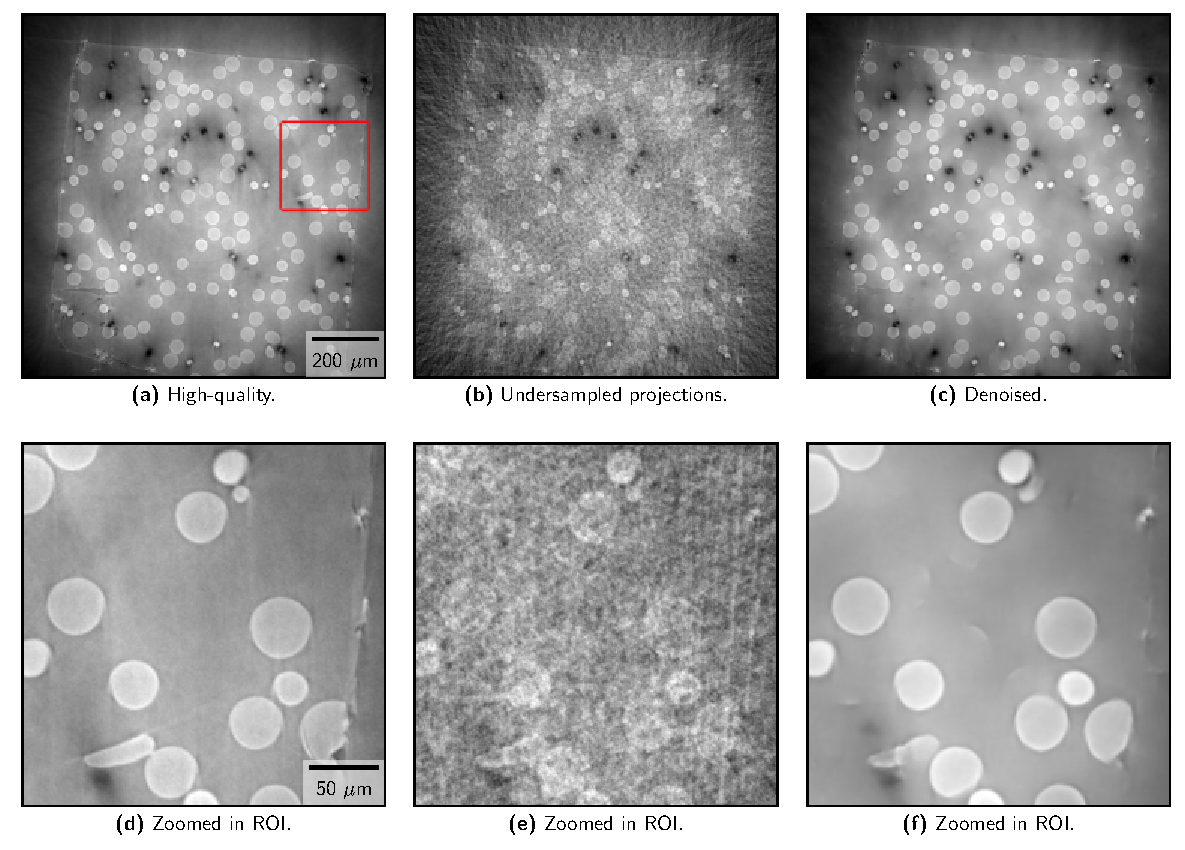
\includegraphics[width=.9\textwidth]{figures/croppeddenoising.pdf}
  \caption[Cropped image denoising]{Denoising of cropped borosilicate glass spheres dataset. Images d), e), and f) are zoomed in \gls{roi}s of images a), b), and c) respectively. The \gls{roi} is marked in a). }
  \label{fig:croppeddenoising}
\end{figure}

\begin{figure}[htbp]
  \centering
  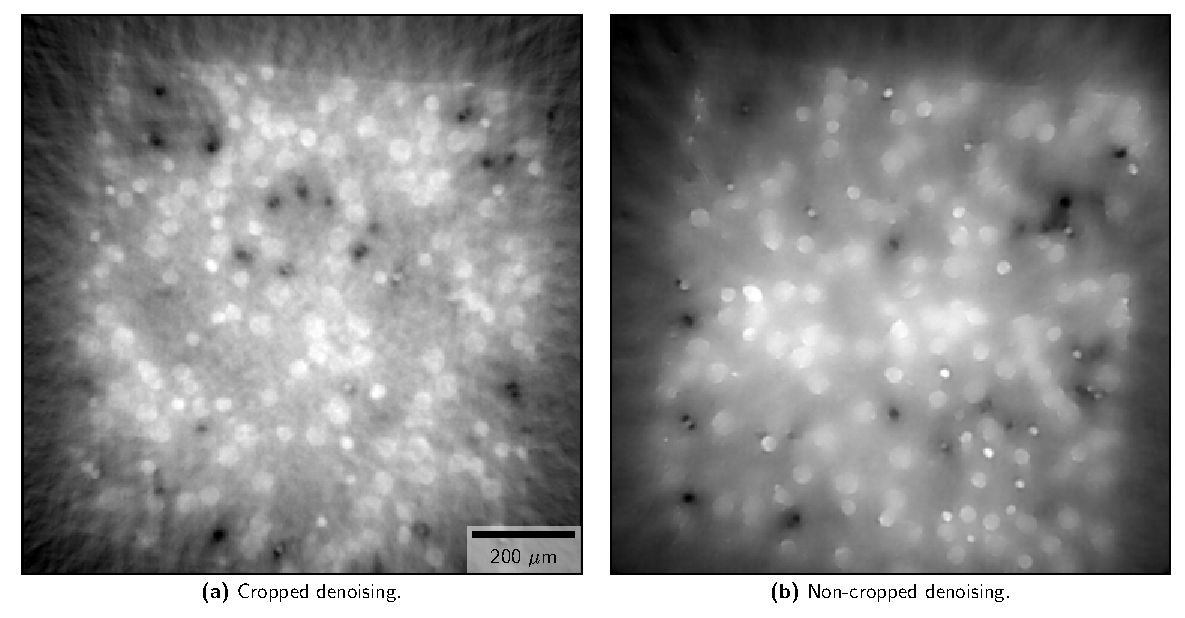
\includegraphics[width=.9\textwidth]{figures/croppednoncroppedearly.pdf}
  \caption[Non-cropped image denoising compared to non-converged cropped image denoising]{Non-cropped image denoising compared to non-converged cropped image denoising. The cropped denoising is after merely $500$ iterations of the same denoising as in \cref{fig:croppeddenoising}. The non-cropped denoising has been cropped after denoising for easier comparison. The two images are of different slices of the same dataset. }
  \label{fig:croppednoncroppedearly}
\end{figure}

\subsection{Hyperparameter and Loss Function Changes}
How the change in the loss function affected the denoising operation was explored for the borosilicate glass spheres dataset. A log-cosh term (see \cref{sec:ml:training:lossfunctions}) was added to the loss function, and the resulting denoised images obtained using different loss functions were compared. All other hyperparameters were kept constant, only the composition of the loss function was changed (i.e. adding log-cosh loss and reducing $\lambda_{\text{MSE}}$). The resulting two denoisings for an arbitrary slice is given in \cref{fig:losschangedenoisingcomparison}. 

\begin{figure}[htbp]
  \centering
  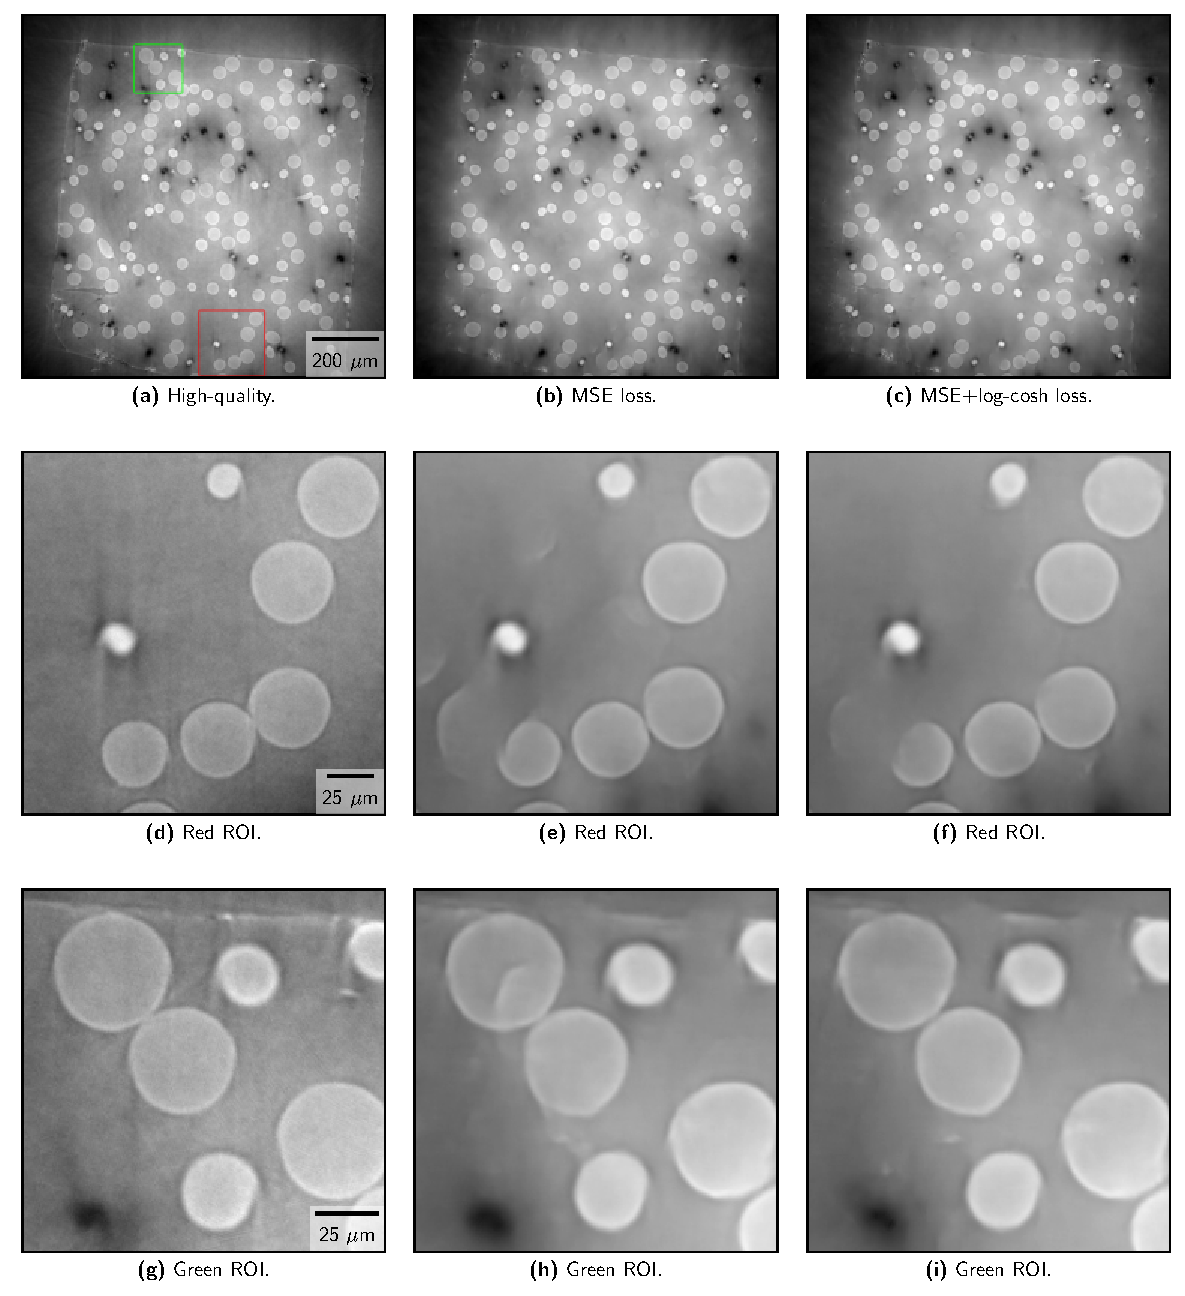
\includegraphics[width=.9\textwidth]{figures/losschangedenoisingcomparison.pdf}
  \caption[Effect on denoising of changing the loss function]{Effect on denoising of changing loss function. Both denoisings are of the borosilicate glass spheres dataset with a subsampling factor of 32. Two \gls{roi}s have been marked in \textbf{(a)}, and can be seen in \textbf{(d)}-\textbf{(i)}. }
  \label{fig:losschangedenoisingcomparison}
\end{figure}

While there is little visual difference in the two denoisings, the denoising containing a log-cosh based loss achieves a slight improvement in the \gls{ssim} score compared to the one without ($0.789$ vs. $0.788$). There is also no measurable difference in the training time of the network when incorporating another loss function. Because of this minor improvement with no discernible drawback, the loss function containing a log-cosh component is chosen as the default loss function for denoising in this thesis. It is possible that a larger improvement may be achievable by further tuning the weights of the different loss functions, as this has not been thoroughly explored. 

\subsection{Loss Function Evolution}
To try and understand how the TomoGAN network is performing during training, the evolution of the loss function and its components was plotted. This is given in \cref{fig:losstomo00058noadv}. We see that the main reduction in the loss of the network happens during early stages of training, especially the first few iterations. In the first $500$ iterations the loss changes from $\approx 7000$ to $\approx 100$, however a denoising after $500$ iterations does not perform well (as is given in \cref{fig:croppednoncroppedearly}a). At $100000$ iterations, the loss is $\approx 70$. In the early iterations the denoising solves for low spatial-frequency features which result in large decreases in the loss function. In later iterations high frequency information is captured, which has a smaller impact on the loss as these are finer details. 

If denoising performance could be gauged based solely on \cref{fig:losstomo00058noadv}, the denoised image after $20000$ iterations should be very similar to after $100000$ iterations. Looking at \cref{fig:iterationdenoisingcomparison} it is evident that this is not correct. The denoising after $20000$ iterations achieves an \gls{ssim} of $0.778$ compared to $0.789$ after $100000$ iterations. After $20000$ iterations, the spheres in the borosilicate glass spheres dataset are less sharp and more artefacts have been introduced. This is consistent with high frequency information being captured at later iterations. How the \gls{ssim} and \gls{mse} of an arbitrary slice of the dataset evolve through training is given in \cref{fig:ssimmseevolution}. 

\begin{figure}[htbp]
  \centering
  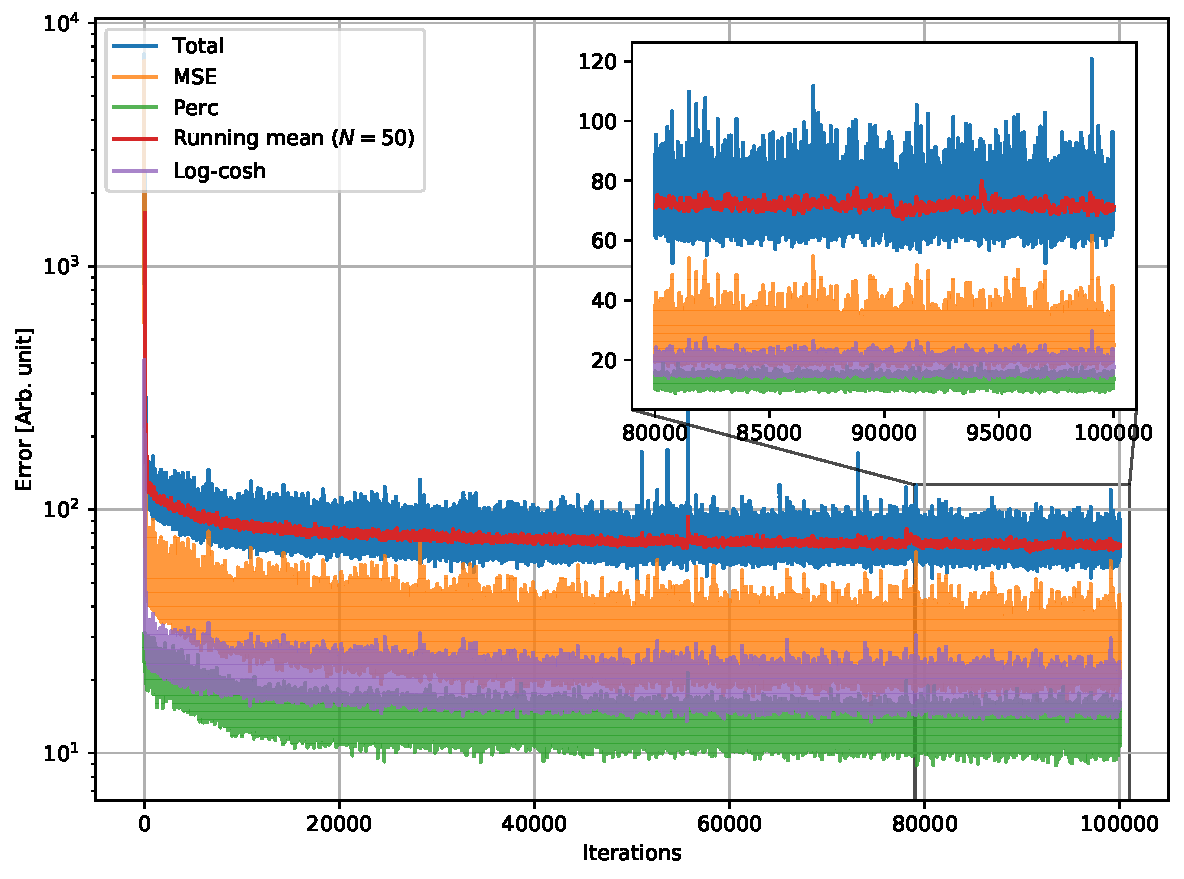
\includegraphics[width=.8\textwidth]{figures/losstomo00058ns32itd4mse035logcosh3depth1.pdf}
  \caption[Loss function evolution during training]{Plot showing how the loss function evolves during $100000$ iterations of training on the borosilicate glass spheres dataset with a subsampling factor of 32. The adversarial loss has been omitted from the plot. The inset axis shows the final $20000$ iterations. Note that the main axis is logarithmic, with the inset axis being linear. The unit of the loss is arbitrary. The running mean is the mean of the previous $50$ values. }
  \label{fig:losstomo00058noadv}
\end{figure}

\begin{figure}[htbp]
  \centering
  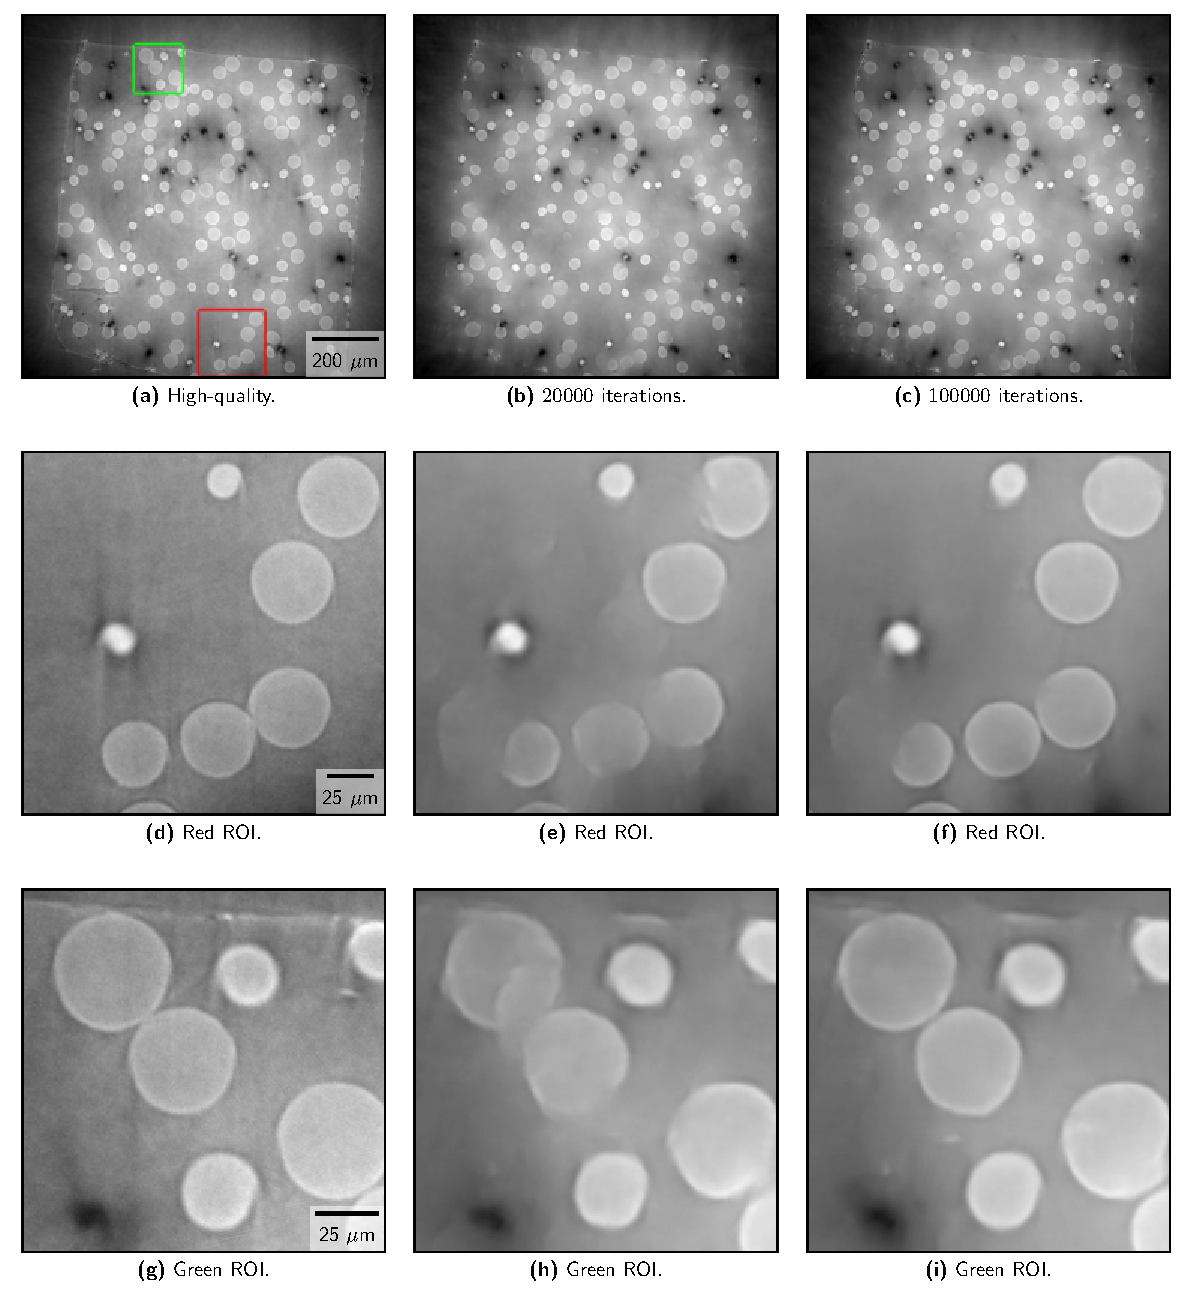
\includegraphics[width=.85\textwidth]{figures/iterationdenoisingcomparison.pdf}
  \caption[Effect on denoising of number of iterations]{Effect on denoising of number of iterations. Both denoisings are of the borosilicate glass spheres dataset with a subsampling factor of 32. Two \gls{roi}s have been marked in \textbf{(a)}, and can be seen in \textbf{(d)}-\textbf{(i)}. The scale bar for \textbf{(a)} applies to \textbf{(b)} and \textbf{(c)}, the scale bar for \textbf{(d)} applies to \textbf{(e)} and \textbf{(f)}, and the scale bar for \textbf{(g)} applies to \textbf{(h)} and \textbf{(i)}. }
  \label{fig:iterationdenoisingcomparison}
\end{figure}

\begin{figure}[htbp]
  \centering
  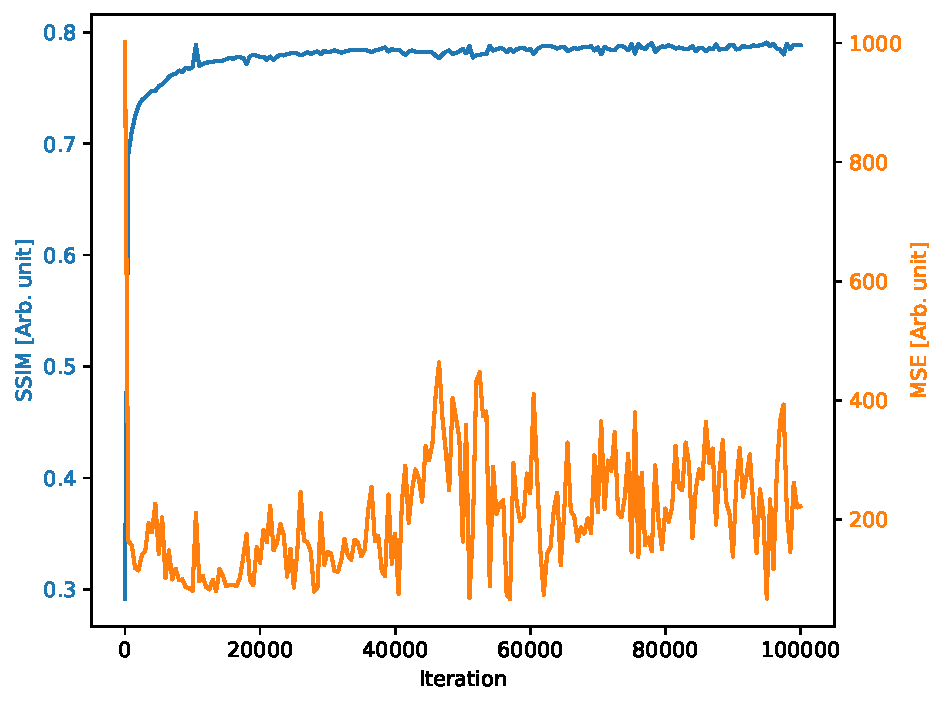
\includegraphics[width=.85\textwidth]{figures/ssimns32logcosh.pdf}
  \caption[SSIM and MSE evolution during training]{Plot showing how the \gls{ssim} and \gls{mse} of an arbitrary slice evolve during $100000$ iterations of training on the borosilicate glass spheres dataset with a subsampling factor of 32. }
  \label{fig:ssimmseevolution}
\end{figure}

\section{Soda Lime Glass Spheres}
The in-house captured dataset \gls{ihlq} of soda lime glass spheres (see \cref{sec:method:datasets:inhouse}) has been denoised using TomoGAN. The network has been trained to try and map the \gls{ihlq} dataset to the \gls{ihhq} dataset. As a comparison, two different reconstruction methods for the \gls{ihlq} dataset have been included: the \gls{fdk} direct reconstruction method and the \gls{piccs} iterative reconstruction method. 

This section focuses on comparing the TomoGAN denoising to using \gls{piccs} for denoising during reconstruction specifically for dynamic \gls{ct} datasets, and also looks at how well 3D information is denoised. 

\subsection{TomoGAN Compared to PICCS}
To compare the TomoGAN denoising to the \gls{ihlq} \gls{piccs} reconstruction, the pixel values along a line on an arbitrary slice of the soda lime glass spheres dataset have been examined. A plot is provided in \cref{fig:kimrobertline}. We see here that the \gls{ihhq} and \gls{ihlq} \gls{piccs} based reconstructions, as well as the denoised \gls{ihlq} dataset, are similar. The \gls{ihlq} \gls{fdk} reconstruction is noisy, and it is hard to clearly discern boundaries. 

\begin{figure}[htbp]
  \centering
  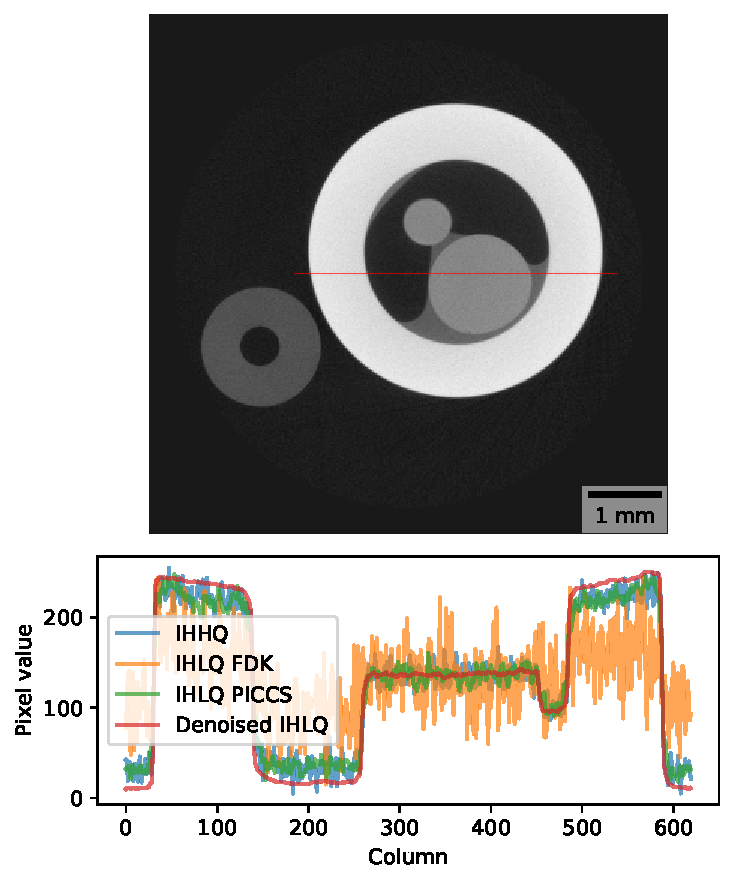
\includegraphics[width=.95\textwidth]{figures/kimrobertline.pdf}
  \caption[Pixel value plot of IHHQ and IHLQ, noisy and denoised]{The plot shows pixel values for 620 pixels on a horizontal line, as shown by the red line on the \gls{hq} image above, on the \gls{ihhq} and \gls{ihlq} dataset, both noisy and denoised. The denoised values are from denoising the \gls{ihlq} \gls{fdk} reconstruction with TomoGAN. }
  \label{fig:kimrobertline}
\end{figure}

This is further confirmed by looking at the histograms of the four different reconstructions and denoisings, provided in \cref{fig:kimroberthist}. Whereas the \gls{ihlq} \gls{piccs} reconstruction is closely related to the \gls{ihhq} reconstruction, it is evident that the \gls{ihlq} \gls{fdk} reconstruction is a gaussian curve, indicating it is primarily noise. No pixel value peaks can be discerned. The histogram of the denoised \gls{ihlq} dataset has peaks similarly located as the \gls{ihhq} dataset, however the peaks are narrower and the dynamic range of the denoised image is increased.\footnote{Dynamic range refers the ratio between the brightest and darkest parts of the image. } The number of peaks in the pixel values for \gls{ihhq} and \gls{ihlq} \gls{piccs} is the same as for the denoised \gls{ihlq}. 


\begin{figure}[htbp]
  \centering
  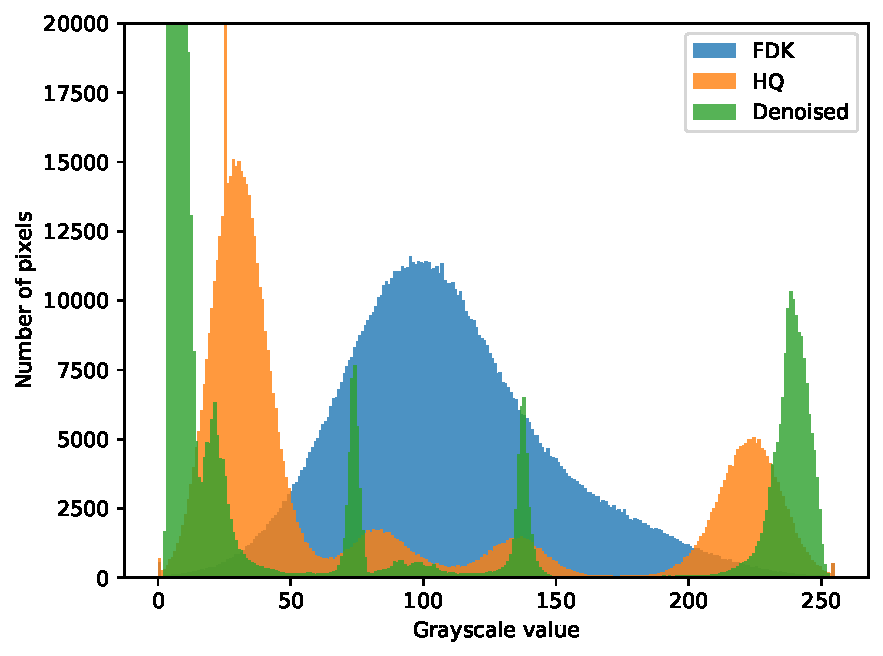
\includegraphics[width=.9\textwidth]{figures/kimroberthist.pdf}
  \caption[Histograms of IHHQ and IHLQ, noisy and denoised]{Histograms of an arbitrary slice from the \gls{ihhq} and \gls{ihlq} \gls{fdk} dataset, both noisy and denoised. The denoised values are from denoising the \gls{ihlq} \gls{fdk} reconstruction with TomoGAN. Note that the ordinate has been cropped to a max value of $20000$. }
  \label{fig:kimroberthist}
\end{figure}

The TomoGAN denoising of the \gls{ihlq} \gls{fdk} reconstruction has captured the boundaries between different materials in the dataset, as can be seen in \cref{fig:kimrobertline}. All boundaries correspond well to the \gls{ihhq} reconstruction. The pixel values within a material are more consistent in the denoised reconstruction than the \gls{ihhq} reconstruction, and we see that the pixel values utilize the available range of values more (i.e. the lowest pixel values are lower, and the highest pixel values are higher). The dynamic range is increased. 


\subsection{Effect of Depth Parameter on 3D Denoising}
For this dataset, the 3D stability of the denoising method has been explored. Because the TomoGAN network uses 2D convolutions (see \cref{sec:method:tomogan}), it is primarily a 2D denoising method. The network allows for 3D information to be included in the denoising by adjusting a depth parameter, which looks at adjacent slices and performs a $1\times1$ convolution across them, however by inspecting the structure of the network (see \cref{fig:tomoganstructure}) it is evident that this 3D information is only used at early stages of the denoising. Only the initial $1\times1$ convolutional layer, before the down sampling part of the network, looks at the depth. 

The result of the limited use of 3D information is that the network has a plane that is the primary focus of the denoising. By inspecting \cref{fig:bigfigure} it is evident that the denoising is done on the axial plane. For a denoising with a depth of 1, it is very clear that there is a lack of consistency between axial planes. Looking at the yellow \gls{roi} there are banding artefacts introduced between the axial layers, interaxial artifacting has been introduced. The same denoising with a depth of 7 still contains some of these interaxial banding artefacts, however the introduction of some 3D knowledge reduces the artifacting. When instead looking at the blue \gls{roi}, which is on the axial plane, there are no banding artefacts. By visual inspection of \cref{fig:bigfigure}, we see that the interaxial banding artifacting is reduced when the depth is increased. The specific depth that yields the best results is dependent on dataset characteristics, such as feature resolution \cite{liu2020tomogan}. 

In the green \gls{roi} in \cref{fig:bigfigure}, we see details that were indistinguishable in the \gls{ihlq} \gls{fdk} reconstruction, and not properly visible in the \gls{ihlq} \gls{piccs} reconstruction, are being captured by TomoGAN. These details are clearly visible when only a depth of 1 is used, however they are highly prone to interaxial banding artefacts between layers, and increasing the depth helps reduce this artifacting. 

\begin{figure}[htbp]
  \centering
  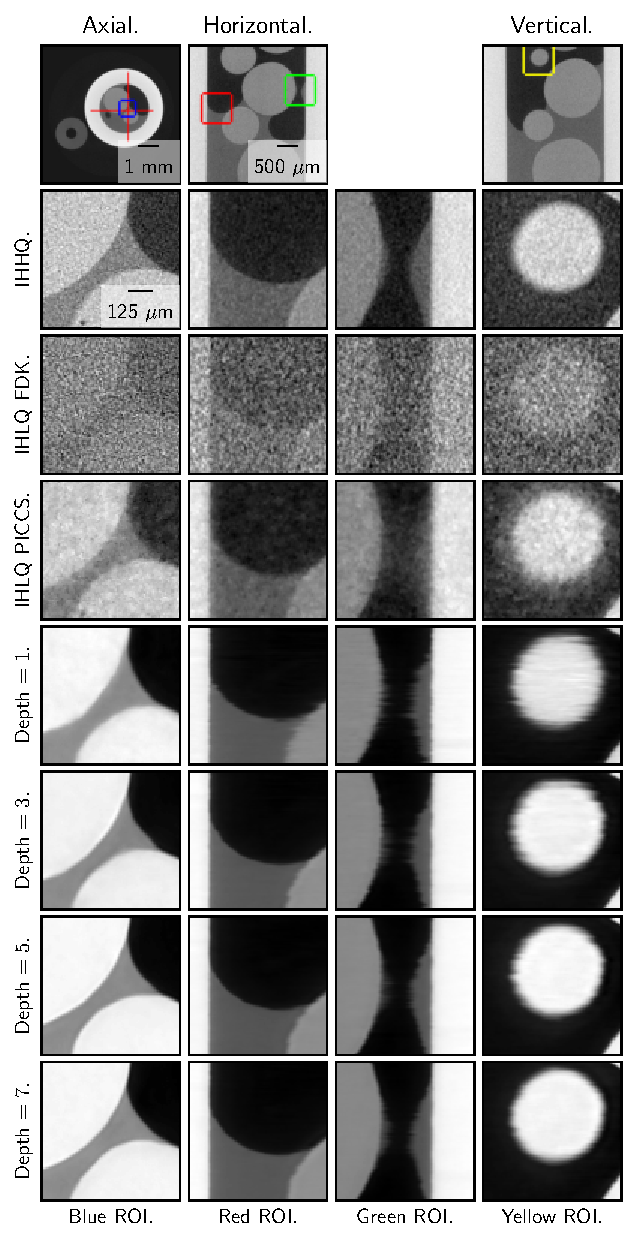
\includegraphics[width=.77\textwidth]{figures/bigfigure.pdf}
  \caption[Different reconstructions and denoisings of the IHLQ and IHHQ datasets]{Different reconstructions and denoisings of the \gls{ihhq} and \gls{ihlq} datasets. The top three images are full views of the \gls{ihhq} dataset. The red horizontal line in the top left figure corresponds to the sagittal view in the top middle figure, and the red vertical line corresponds to the coronal view in the top right figure. Four \glspl{roi} have been marked in the top figures and have been zoomed in for the different reconstructions and denoisings. All zoomed in figures have the same scale bar. }
  \label{fig:bigfigure}
\end{figure}


\section{Pierre Shale}
The Pierre shale dataset (see \cref{sec:method:datasets:shale}) does not have a corresponding high-quality dataset available. It was therefore denoised using TomoGAN trained on different datasets. 

This section looks at the performance of TomoGAN when a corresponding high-quality dataset is not available. 

\subsection{Denoising Without High-quality Dataset}
Because a high-quality imaging of the same dataset is unavailable, four different datasets were used to train TomoGAN to attempt to denoise the Pierre shale dataset. An overview of the datasets used to train for denoising is provided in \cref{tab:pierreshaledenoisingdetails}, and the corresponding denoisings for an arbitrary slice of the dataset are provided in \cref{fig:shale}. 

Denoising A is performed with a network not trained on a shale dataset, and denoisings B-D are performed with a network trained on shale denoising. 

\begin{table}[htbp]
  \centering
  \caption[Pierre shale denoising details]{Pierre shale denoising details. tomo\_00058 is the borosilicate glass spheres dataset, and tomo\_00001 and tomo\_00002 are two shale datasets from TomoBank (see \cref{sec:method:datasets:tomo00058}). The altered scaling in the pre-processing (see \cref{sec:method:compilingdataset}) of denoising D corresponds to changing the maximum and minimum pixel values used to crop the pixel values in an image. }
  \label{tab:pierreshaledenoisingdetails}
  \begin{tabular}{lll}
  \hline
  Denoising name & Training dataset & Pre-processing\\
  \hhline{===}
  Denoising A & tomo\_00058 & Standard \\
  Denoising B & tomo\_00001 & Standard \\
  Denoising C & tomo\_00002 & Standard \\
  Denoising D & tomo\_00002 & Altered scaling \\
  \hline
  \end{tabular}
\end{table}

\begin{figure}
  \begin{subfigure}[t]{\textwidth}
    \centering
    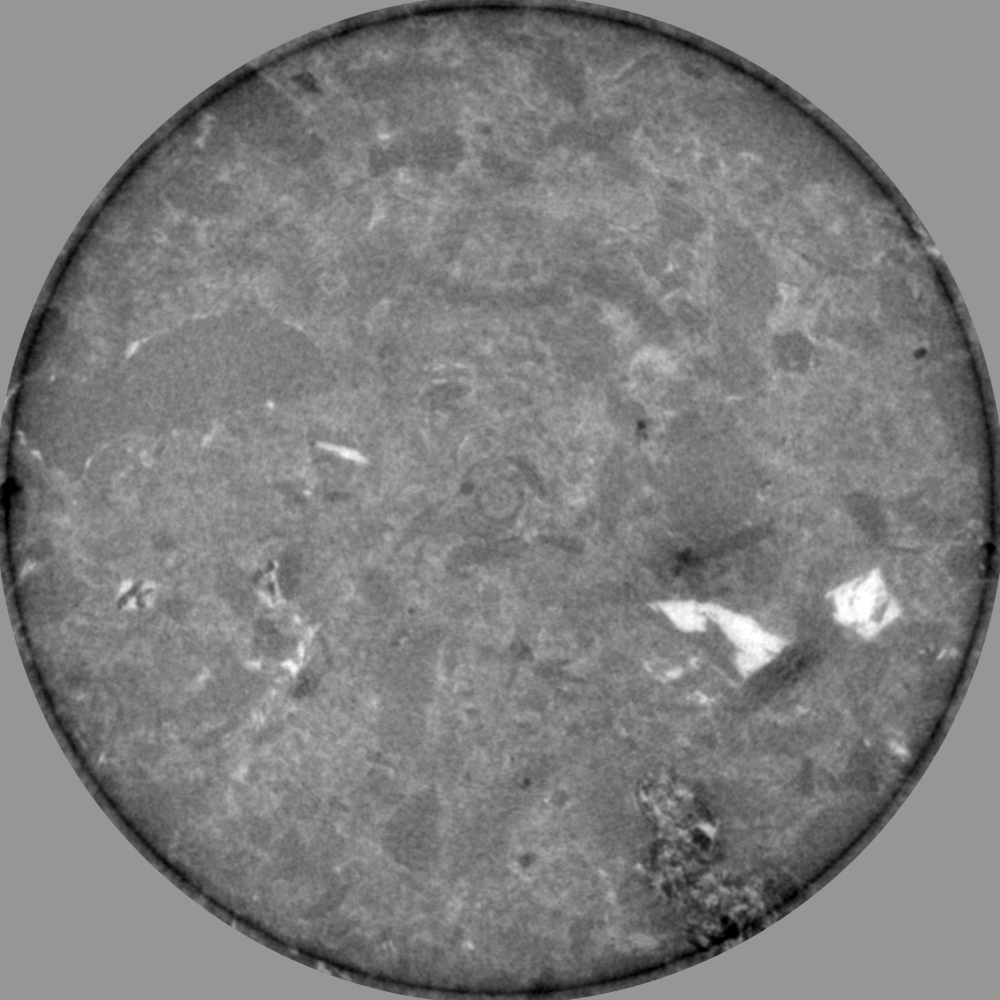
\includegraphics[width=.45\textwidth]{figures/shale/shale_ns/0.png}
    \caption{Original image. }
  \end{subfigure}

  \medskip

  \begin{subfigure}[t]{.45\textwidth}
    \centering
    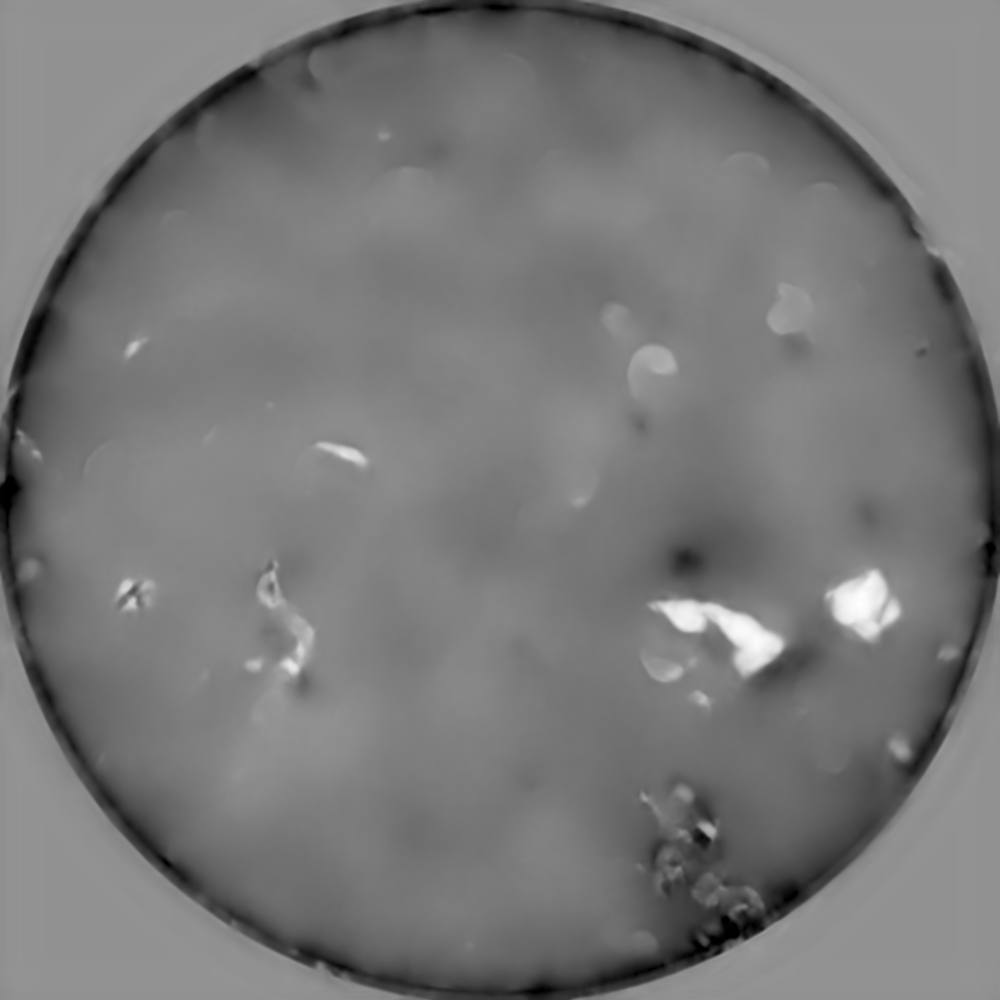
\includegraphics[width=\linewidth]{figures/shale/shale_dn_tomo00058/0.png}
    \caption{Denoising A. }
  \end{subfigure}
  \hfill
  \begin{subfigure}[t]{.45\textwidth}
    \centering
    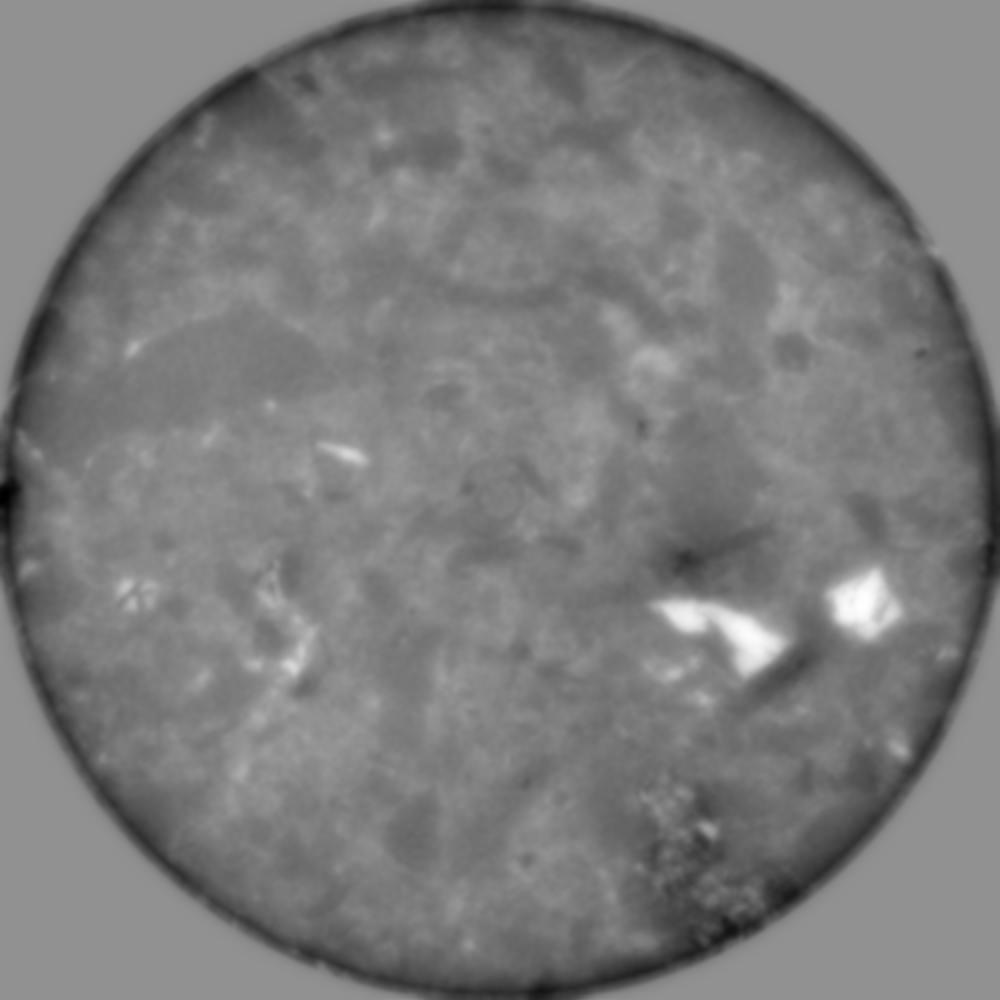
\includegraphics[width=\linewidth]{figures/shale/shale_dn_tomo00001/0.png}
    \caption{Denoising B. }
  \end{subfigure}

  \medskip

  \begin{subfigure}[t]{.45\textwidth}
    \centering
    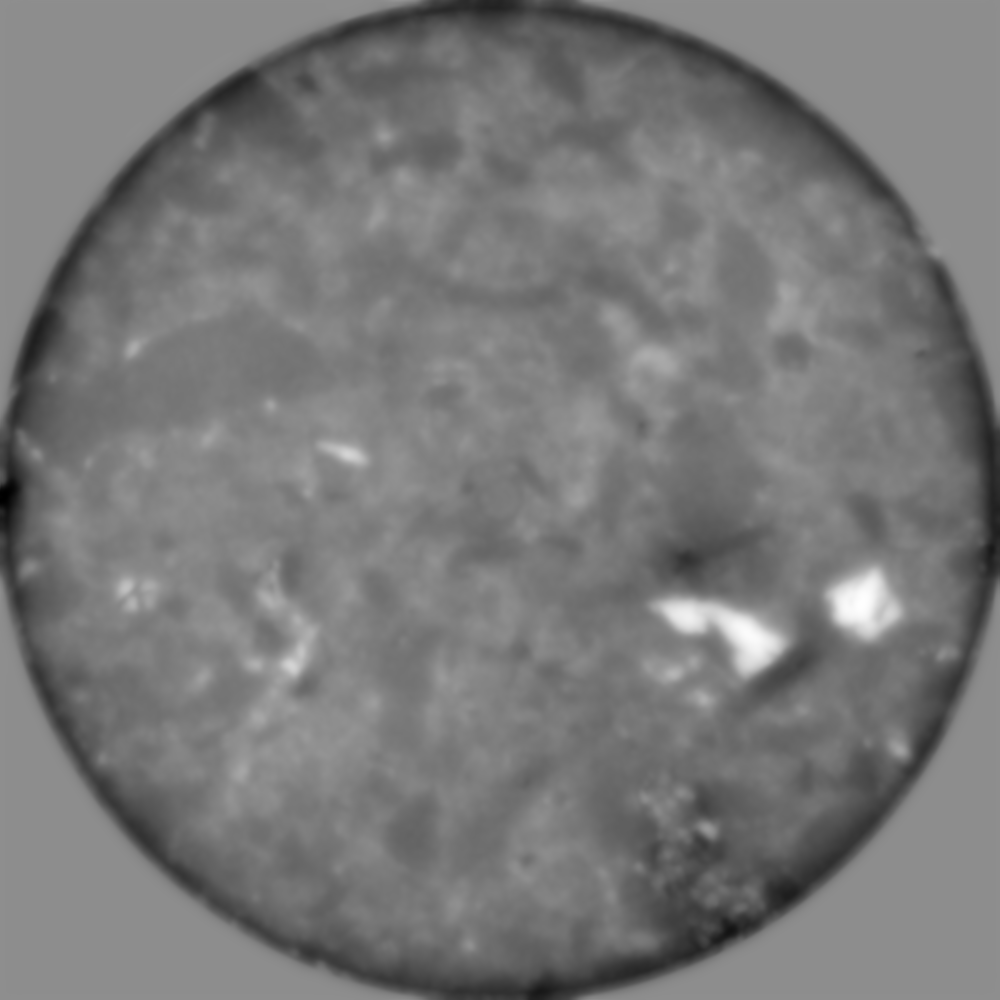
\includegraphics[width=\linewidth]{figures/shale/shale_dn_tomo00002/0.png}
    \caption{Denoising C. }
    \label{fig:shale:c}
  \end{subfigure}
  \hfill
  \begin{subfigure}[t]{.45\textwidth}
    \centering
    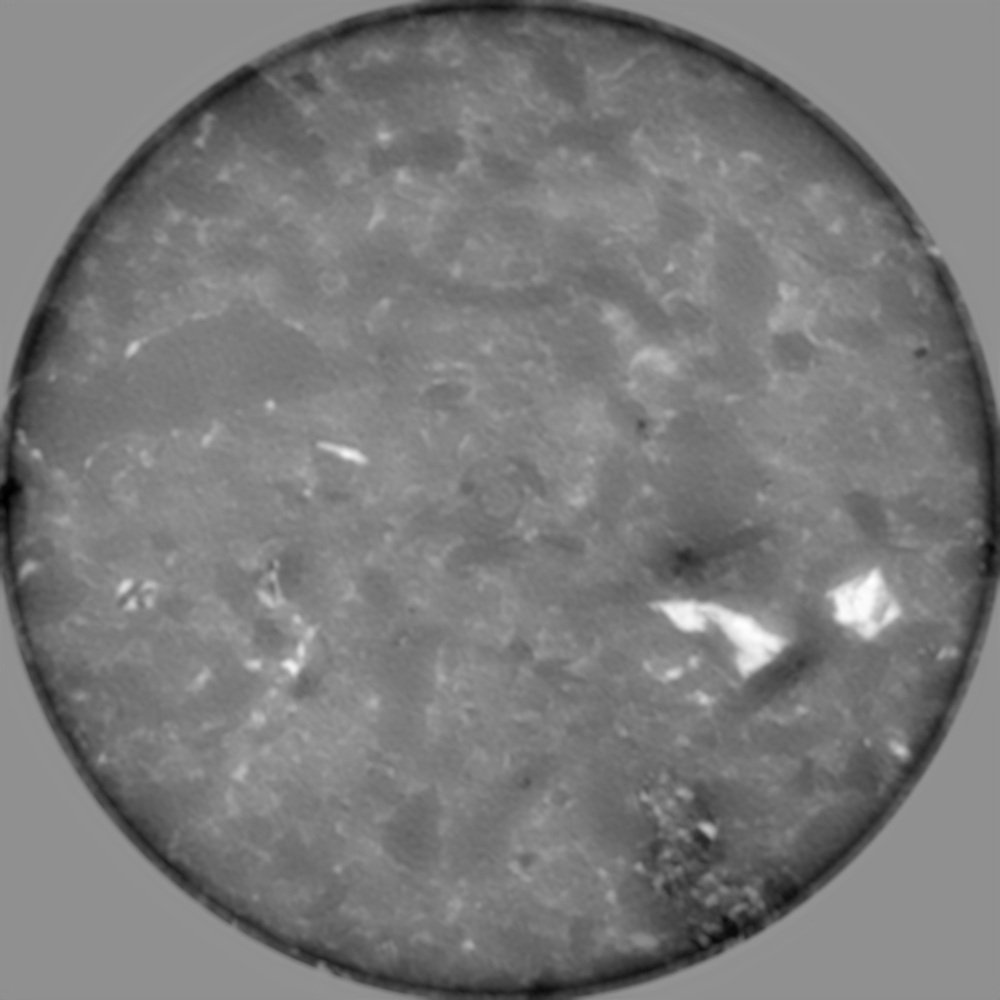
\includegraphics[width=\linewidth]{figures/shale/shale_dn_tomo00002min7/0.png}
    \caption{Denoising D. }
    \label{fig:shale:d}
  \end{subfigure}
  \caption[Attempted Pierre shale denoising without a corresponding high-quality dataset]{Attempted Pierre shale denoising without a corresponding high-quality dataset. The subfigure captions refer to different trainings of TomoGAN (see \cref{tab:pierreshaledenoisingdetails}). }
  \label{fig:shale}
\end{figure}

From \cref{fig:shale} we see that none of the four different denoisings perform well, with denoising A (corresponding to the network trained for the borosilicate glass spheres dataset) performing the worst. All denoisings cause blurring of the images. This is further confirmed by looking at the histograms of the images, which is provided in \cref{fig:shalehistogram}. All histograms contain a large spike corresponding to the gray area around the sample, as well as a gaussian curve indicating noise or poor segmentation. No clear spikes in the pixel values can be distinguished for any of the denoisings, nor the original image. 

\begin{figure}[htbp]
  \centering
  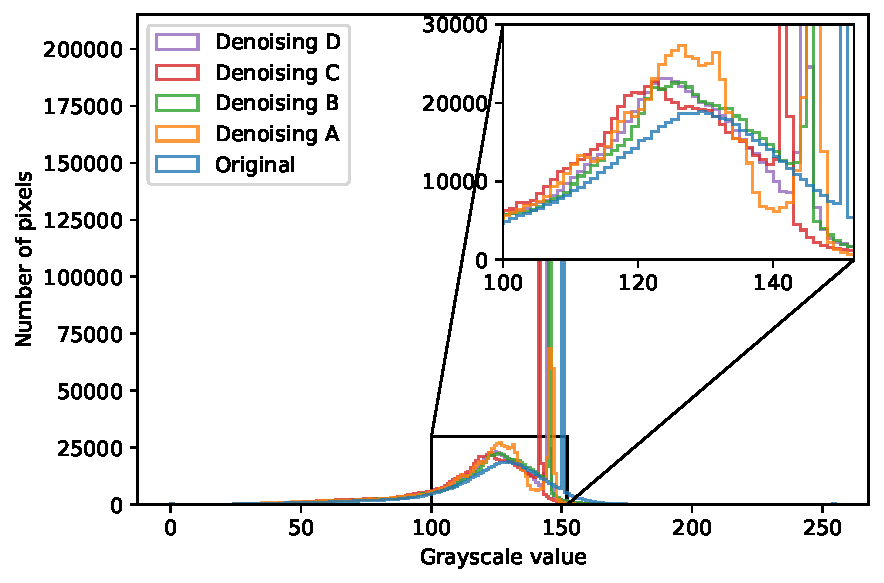
\includegraphics[width=.9\textwidth]{figures/shalehistogram.pdf}
  \caption[Histogram of Pierre shale denoisings]{Histogram of Pierre shale denoisings. The inset axis contains a zoomed in plot with the ordinate cropped to $30000$. See \cref{tab:pierreshaledenoisingdetails} for details on the labels in the legend. }
  \label{fig:shalehistogram}
\end{figure}

Based on these observations, it seems likely that denoising requires finding a similar training dataset. Based on visual inspection of \cref{fig:shale}, the denoising using the network trained on the borosilicate glass spheres dataset performs poorly, and the other three denoisings using shale datasets all achieve better results, though still not of sufficient quality for further analysis. If a training dataset more similar to the Pierre shale dataset were available, the denoising results may be improved significantly. Changing the pre-processing steps may also further improve the denoising results, as indicated by visual inspection of \cref{fig:shale:c,fig:shale:d}, where the latter causes less blurring even though both are trained on the same dataset with only a change in the pre-processing. The TomoGAN network has been reported to work for denoising shale datasets \cite{liu2020tomogan}. 